\documentclass[a4paper, 
	twoside, 
	12pt, 
	toc=bibliographynumbered, 
	numbers=noendperiod, 
	ngerman,
	openany, 
	fleqn]{scrbook}

%#### Meine Eingabedaten #######################################

% die nachfolgenden Werte m�ssen bei jeder Arbeit angepasst werden

\def\ausarbeitungsTyp{Master Thesis} %oder Masterarbeit
\def\meineArbeitsnummer{6843331}
\def\meinStudiengang{Informatik}
\def\meinErstellungsdatum{DD.MM.YYYY} % z.B. 24.01.2012
\def\meinTitel{Evaluation and Implementation of a motivational bot to
support documentation process in mechatronics
system design}
\def\meinName{Michael Mayflower}
\def\meineMatrikelnummer{}
\def\meinErstgutachter{Prof. Dr.-Ing. Roman Dumitrescu} % auch bei Seminaren
\def\meinZweitgutachter{Prof. Dr. Eyke H\"ullermeier} % bei Seminaren irrelevant
\def\meinErstBetreuer{Name Betreuer}
\def\meinZweitBetreuer{Name Betreuer}
\def\meineFirma{FIRMA} %In Gro�buchstaben!
\def\meineFirmaAdresse{Adresse Firma} % mit \\ getrennt


%###############################################################

%%%%%%%%%%%%%%%%%%%%%%%%%%%%%%%%%%%%%%%%%%%%%%%%%%%%%%%%%%%%%%
% Schrift / Sprache
%%%%%%%%%%%%%%%%%%%%%%%%%%%%%%%%%%%%%%%%%%%%%%%%%%%%%%%%%%%%%%,UKenglish,USenglish,english,american
\usepackage[american]{babel}
\usepackage[utf8]{inputenc} 
\usepackage{mathptmx}
\usepackage[scaled=0.92]{helvet}

\usepackage[nolist]{acronym}



\setlength\emergencystretch{5em}
\usepackage{microtype}

%%%%%%%%%%%%%%%%%%%%%%%%%%%%%%%%%%%%%%%%
% Seitenlayout
%%%%%%%%%%%%%%%%%%%%%%%%%%%%%%%%%%%%%%%%
\usepackage{scrpage2}

\pagestyle{scrheadings}
\clearscrheadfoot
\automark[chapter]{chapter} %Kapitelname oben innen	
\renewcommand*{\headfont}{\normalfont}
\ohead{\pagename~\pagemark}
\rehead{\chaptername~\thechapter}%Kapitelnummer   	
\lohead{\headmark}	%Eintrag: Kopfzeile rechte Seite links oben 															  
\renewcommand*{\chaptermarkformat}{}					
\setheadsepline{0.2pt} %Trennlinie zwischen Kopf und Textkörper
\addtokomafont{pageheadfoot}{\small\rmfamily}%Seitenkopf- und Fußbeschriftung in small
\renewcommand*{\chapterpagestyle}{scrheadings}	%normaler Kopfzeilenstil für Chapterseiten
\usepackage[justification=centering]{caption}
\captionsetup{skip=0.333\baselineskip}
\usepackage[left=3.0cm,right=3.0cm,top=3.0cm,bottom=2.5cm,includeheadfoot]{geometry} 

%%%%%%%%%%%%%%%%%%%%%%%%%%%%%%%%%%%%%%%%
% Überschriften und Inhaltsverzeichnis
%%%%%%%%%%%%%%%%%%%%%%%%%%%%%%%%%%%%%%%%
\usepackage{tocloft}%für Inhaltsverzeichnis
\usepackage{titlesec}%Ändern der überschriften

\usepackage{listings}
\usepackage{color}
\definecolor{dkgreen}{rgb}{0,0.6,0}
\definecolor{gray}{rgb}{0.5,0.5,0.5}
\definecolor{mauve}{rgb}{0.58,0,0.82}

\lstset{frame=tb,
  language=python,
  aboveskip=3mm,
  belowskip=3mm,
  showstringspaces=false,
  columns=flexible,
  basicstyle={\small\ttfamily},
  numbers=none,
  numberstyle=\tiny\color{gray},
  keywordstyle=\color{blue},
  commentstyle=\color{dkgreen},
  stringstyle=\color{mauve},
  breaklines=true,
  breakatwhitespace=true,
  tabsize=3
}
\usepackage[justification=centering]{caption}
\setcounter{secnumdepth}{3}
\titleformat{\chapter}[hang]{\large\sffamily\bfseries}{\thechapter\quad}{1cm}{}
\titleformat{\section}[hang]{\fontsize{13pt}{16pt}\selectfont\sffamily\bfseries}{\thesection\quad}{1.2cm}{}
\titleformat{\subsection}[hang]{\normalsize\sffamily\bfseries}{\thesubsection\quad}{1cm}{}
\titleformat{\subsubsection}[hang]{\normalsize\sffamily\mdseries}{\thesubsubsection\quad}{1cm}{}
\addtokomafont{chapter}{\large}
%\addtokomafont{section}{\fontsize{13pt}{16pt}\selectfont}
%\addtokomafont{subsection}{\normalsize}
%\addtokomafont{subsubsection}{\normalsize\mdseries}
\renewcommand*{\cftchapfont}{}
\renewcommand*{\cftsecfont}{}
\renewcommand*{\cftsubsecfont}{}
\renewcommand*{\cftchappagefont}{}
\renewcommand*{\cftsecpagefont}{}
\renewcommand*{\cftsubsecpagefont}{}
\renewcommand{\cftchapleader}{\cftdotfill{3.0}}
\renewcommand{\cftsecleader}{\cftdotfill{3.0}}
\renewcommand{\cftsubsecleader}{\cftdotfill{3.0}}

\setlength{\beforetitleunit}{9pt}
\setlength{\aftertitleunit}{0pt}
\titlespacing{\chapter}{0pt}{1.0\beforetitleunit plus0.25\beforetitleunit minus0.25\beforetitleunit}{1.0\aftertitleunit plus0.1\aftertitleunit minus0.25\aftertitleunit} %Abstand. vor und nach
\titlespacing{\section}{0pt}{1.0\beforetitleunit plus0.25\beforetitleunit minus0.25\beforetitleunit}{1.0\aftertitleunit plus0.1\aftertitleunit minus0.25\aftertitleunit} %Abstand. vor und nach Section
\titlespacing{\subsection}{0pt}{0.8\beforetitleunit plus0.1\beforetitleunit minus0.1\beforetitleunit}{0.8\aftertitleunit plus0.1\aftertitleunit minus0.25\aftertitleunit}	%Abstand vor und nach Subsection
\titlespacing{\subsubsection}{0pt}{0.6\beforetitleunit plus0.1\beforetitleunit minus0.1\beforetitleunit}{0.6\aftertitleunit plus0.1\aftertitleunit minus0.1\aftertitleunit}
\titlespacing{\paragraph}{0pt}{0.4\beforetitleunit plus0.1\beforetitleunit minus0.1\beforetitleunit}{0.5\beforetitleunit}

%%%%%%%%%%%%%%%%%%%%%%%%%%%%%%%%%%%%%%%%
% PDF-Einstellungen Hyperref
%%%%%%%%%%%%%%%%%%%%%%%%%%%%%%%%%%%%%%%%
% ueberpruefen, ob wir pdflatex ausfuehren (geht nur bei Koma-Klassen)
\ifpdfoutput
{
% PDF wird genutzt
	
	\usepackage[pdftex]{graphicx}
	% eigene Farben für Links:
  	%\definecolor{myLinkColor}{rgb}{0,0,.5}
  	%\definecolor{myCiteColor}{rgb}{0,.5,0}
  	%\definecolor{myFileColor}{rgb}{.5,0,0}
  	%\definecolor{myURLColor}{rgb}{0,0,1}
  	% Setzen aller Link-Farben auf Schwarz 
  	\definecolor{myLinkColor}{rgb}{0,0,0}
  	\definecolor{myCiteColor}{rgb}{0,0,0}
  	  	  	\definecolor{myFileColor}{rgb}{0,0,0}
  	  	  	\definecolor{myURLColor}{rgb}{0,0,0}
  	\usepackage[pdftex,%
  	  		plainpages=false,%
  	  		pdfpagelabels,% Seitenzahl als z.B. 'ii (4 of 40)' anstatt '4 of 40' darstellen
  	  		colorlinks=true,%
  	  		linkcolor=myLinkColor,%
  	  		citecolor=myCiteColor,%
  	  		filecolor=myFileColor,%
  	  		urlcolor=myURLColor,%
  	  		bookmarks,% Lesezeichen erstellen
  	  		bookmarksnumbered, % Lesezeichen nummeriert wie im Inhaltsverzeichnis
  	  		breaklinks, % Zeilenumbrüche bei Links erlauben
  			unicode
  	  		%pdfpagelayout={TwoColumnRight}% zweiseitiges fortlaufendes Layout
  	  		]{hyperref}
}
{
% Kein PDF  
  	\usepackage{graphicx}
  %	\usepackage{color}
  	\usepackage[hypertex, 
  		bookmarks,% Lesezeichen erstellen
  		bookmarksnumbered, % Lesezeichen nummeriert wie im Inhaltsverzeichnis
  		breaklinks, % Zeilenumbrüche bei Links erlauben
  		]{hyperref}
  \DeclareGraphicsExtensions{.eps,.ps} % Dateiendungen für Grafikdateien
}    



%%%%%%%%%%%%%%%%%%%%%%%%%%%%%%%%%%%%%%%%%%%%%%%%%%%%%%%%%%%%%
%
%  Mathe-Pakete
%
%%%%%%%%%%%%%%%%%%%%%%%%%%%%%%%%%%%%%%%%%%%%%%%%%%%%%%%%%%%%%%
\usepackage{amsfonts} 	% extra math fonts
\usepackage{amsmath} 	% mathematical formulas
\usepackage{amssymb} 	% Symbole für Zahlenmengen usw.
\titleformat{\paragraph}
{\normalfont\normalsize\bfseries}{\theparagraph}{1em}{}
\titlespacing*{\paragraph}
{0pt}{3.25ex plus 1ex minus .2ex}{1.5ex plus .2ex}

%%%%%%%%%%%%%%%%%%%%%%%%%%%%%%%%%%%%%%%%
% Body
%%%%%%%%%%%%%%%%%%%%%%%%%%%%%%%%%%%%%%%%
\renewcommand{\baselinestretch}{1.12}
\parindent0.0cm	% Einrückung bei Absatz auf 0 setzen
\parskip\medskipamount %Legt den Abstand zwischen den nachfolgenden Absätzen fest
\setlength{\mathindent}{1.25cm} %Einrückung der Formeln

%% snake-oil für den Satz
\pretolerance=100           %% Textsatz: interner Parameter zur Steuerung des Zeilenumbruchs
\tolerance 300              %% 1414 Bewertungsgrenzwert für schlecht umbrochene Zeilen
\hfuzz=0.2pt                %% Grenze, ab der eine overfull hbox gemeldet wird
\vfuzz=0.2pt                %% Grenzwert, ab dem die Überfüllung einer \vbox protokolliert wird
\hbadness 1414              %% Grenzwert für »schlechte« Zeilen, bzw. Boxen
\vbadness	1000            %% Grenzwert für eine »schlechte« \vbox 
\emergencystretch 1em       %% zusätzlicher dynamischer Leerraum
\hyphenpenalty=30           %% Strafpunkte bei Silbentrennung über Absatz hinweg
\widowpenalty=100000        %% falls letzte Zeile auf neue Seite gebrochen wird.
\clubpenalty=100000         %% wenn erste Zeile eines Absatzes auf alter Seite bleibt.
\doublehyphendemerits=50    %% Aufeinanderfolgende Silbentrennungen eher vermeiden. 
%%%%%%%%%%%%%%%%%%%%%%%%%%%%%%%%%%%%%%%%%%%%%%%%%%%%%%%%%%%%%%
%
%  Bilder / Farben etc.
%
%%%%%%%%%%%%%%%%%%%%%%%%%%%%%%%%%%%%%%%%%%%%%%%%%%%%%%%%%%%%%%
\usepackage{graphicx}		% Einbinden von Bildern / Enhanced support for graphics
\usepackage{color}			% Colour control for LaTeX documents.
\usepackage[tight,TABTOPCAP]{subfig}%Figures broken into subfigures, Alternative "subcaption"
%\usepackage{wallpaper}		% Easy addition of wallpapers (background images) to LaTeX documents, including tiling
% \usepackage{lscape}		% Place selected parts of a document in landscape
% \usepackage{rotating} 	% Rotation tools, including rotated full-page floats

%Name für Bildunterschriften/Tabellenüberschriften
\renewcaptionname{ngerman}{\figurename}{\itshape Bild}
\renewcaptionname{ngerman}{\tablename}{\itshape Tabelle}

%Format der Nummerierungen
\renewcommand{\thefigure}{\arabic{chapter}-\arabic{figure}}
\renewcommand{\thetable}{\arabic{chapter}-\arabic{table}}
\renewcommand{\theequation}{\arabic{chapter}-\arabic{equation}} 

% Formatierung der Bildunterschrift im Blocksatz (nicht zentriert) und mit zusätzlichem Tab nach dem Label
\DeclareCaptionFormat{myformat}{#1#2\quad#3}
\captionsetup{singlelinecheck=false,justification=centering,font=it, labelfont=it,format = myformat}

%%%%%%%%%%%%%%%%%%%%%%%%%%%%
% TEST
%%%%%%%%%%%%%%%%%%%%%%%%%%%%%

%\usepackage{minitoc}% für extra Inhaltsverzeichnisse

\usepackage{bibgerm}
\usepackage{amsmath}
\usepackage{amssymb}

%%%%%%%%%%%%%%%%%%%%%%%%%%%%%%%%%%%%%%%%
% Beginn Dokument
%%%%%%%%%%%%%%%%%%%%%%%%%%%%%%%%%%%%%%%%
\begin{document}
\frontmatter


%%%%%%%%%%%%%%%%%%%%%%%%%%%%%%%%%%%%%%%%
% Titelseite
%%%%%%%%%%%%%%%%%%%%%%%%%%%%%%%%%%%%%%%
\begin{titlepage}
\newgeometry{left=30mm, right=30mm, top=10mm, bottom=5mm}
\begin{figure}[htb]
\centering
\begin{addmargin*}[0cm]{0cm} % negativer Parameter verringert den Rand
\begin{minipage}[b]{0.5\textwidth} % [b] => Ausrichtung an \caption
\flushleft
  
\includegraphics[width=0.6\textwidth]{figures/HNI.png}
\end{minipage}
\hspace{.01\linewidth}
\begin{minipage}[b]{.5\textwidth}
\begin{addmargin*}[0cm]{-0.5cm} % negativer Parameter verringert den Rand
\flushright
  
\includegraphics[width=0.5\textwidth]{figures/iem.jpg}
\end{addmargin*}
 \end{minipage}
\end{addmargin*}

 \end{figure}
\sffamily
%\huge

\vspace*{3.5cm}
\fontsize{24pt}{26pt}\selectfont
\begin{center}
\textbf{\ausarbeitungsTyp}


\Large
\textbf{\meinTitel}
\vspace*{3cm}

\normalsize
Presented by
\vspace*{0.5cm}

cand. Bhargavi Mohan

Matr.-Nr. 6843331 
\vspace*{1.5cm}

\large
\textbf{~}
%\textbf{Nicht Freigegeben}
\end{center}
\vspace*{2cm}
\normalsize
Supervisor:

\begin{tabbing}
\quad\=Formel\quad\= Formel\quad\= Formel\quad\= Formel\quad\= Formel\quad\= Formel \quad\= Formel\quad\= Formel\kill  
\meinErstgutachter\\
\meinZweitgutachter \>\>\>\>\>\>\> Paderborn, 24.05.2021
%\meinErstBetreuer\\
%\meinZweitBetreuer \>\>\>\>\>\>\> Paderborn, \meinErstellungsdatum
\end{tabbing}
\normalsize
\vfill
\newpage
%----------------------------------------------------Seite2
\thispagestyle{empty}    %keine Nummerierung
\vspace*{16.5cm}

\ausarbeitungsTyp~  Nr. (MA0188)

\vspace*{1cm}
\textbf{\meinTitel}
\vspace*{0.25cm}

am: 24.05.2021

\makebox[8cm][l]{
\hspace{-3mm}
\parbox[t]{7.3cm}{
\begin{flushleft}

\rmfamily{\textbf{FRAUNHOFER-INSTITUT F\"UR ENTWURFSTECHNIK MECHATRONIK IEM}}


\sffamily \small Projektgruppe Entwurfstechnik\\
Zukunftsmeile 1\\
D-33102 Paderborn\\
\end{flushleft}
}}
\makebox[7.5cm][r]{
\parbox[t]{7cm}{
%\begin{flushleft}
%\rmfamily{\textbf{\meineFirma}}
%
%\sffamily \small \meineFirmaAdresse
%\end{flushleft}
}}

\vfill
\end{titlepage}


%%%%%%%%%%%%%%%%%%%%%%%%%%%%%%%%%%%%%%%%
% Sperrvermerk
%%%%%%%%%%%%%%%%%%%%%%%%%%%%%%%%%%%%%%%%
\thispagestyle{empty}    %keine Nummerierung
\vspace*{8cm}
%\Large
\fontsize{16pt}{18pt}\selectfont
\begin{center}
\sffamily
\bfseries
Blocking notice 
\vspace*{1cm}

This work remains closed to the public due to confidential data and information.
\end{center}
\vspace*{7.5cm}
\normalsize
\sffamily
	\begin{center}
		\begin{tabular}{l l r}
		  \cline{1-1} \cline{3-3}
		  \begin{minipage}[t]{0.5\textwidth}
		    \centering
		    Prof. Dr.-Ing. Roman Dumitrescu
			\end{minipage}
			&
			\begin{minipage}[t]{0\textwidth}
			\end{minipage}
			&
			\begin{minipage}[t]{0.5\textwidth}
			  \centering
			  Bhargavi Mohan
			\end{minipage}
		\end{tabular}
	\end{center}
\cleardoublepage

%%%%%%%%%%%%%%%%%%%%%%%%%%%%%%%%%%%%%%%%
% Erklärung
%%%%%%%%%%%%%%%%%%%%%%%%%%%%%%%%%%%%%%%%
\thispagestyle{empty}    %keine Nummerierung
\newgeometry{left=30mm, right=30mm, top=30mm, bottom=0mm}
\sffamily
\vspace*{16cm}
\textbf{Eidesstattliche Erkl\"arung:}
\parskip 12pt

Hiermit erkl\"are ich an Eides Statt, dass ich die vorliegende Arbeit selbstst\"andig und ohne unerlaubte fremde Hilfe angefertigt, keine anderen als die angegebenen Quellen und Hilfsmittel benutzt und die den benutzten Quellen w\"ortlich oder inhaltlich entnommenen Stellen als solche kenntlich gemacht habe.

\vspace*{2.4cm}

		\begin{tabular}{l}
		  \cline{1-1}
		  \begin{minipage}[t]{0.5\textwidth}
		    
		    Paderborn, 31.05.2021
			\end{minipage}
		\end{tabular}
%\vfill
\cleardoublepage

\thispagestyle{empty}    %keine Nummerierung
\normalsize

\sffamily
\textbf{Abstract}

while working towards a common goal

\rmfamily

%%%%%%%%%%%%%%%%%%%%%%%%%%%%%%%%%%%%%%%%
% Abstract
%%%%%%%%%%%%%%%%%%%%%%%%%%%%%%%%%%%%%%%%
\newpage
\thispagestyle{empty}    %keine Nummerierung
\normalsize

\sffamily
\textbf{}

\rmfamily


\cleardoublepage


\restoregeometry

\mainmatter	%Beginn Hauptteil%

\mainmatter	%Beginn Hauptteil%

\tocloftpagestyle{scrheadings}
\ihead{\contentsname}
\sffamily %Inhaltsverzeichnis in Arial	
\renewcommand*{\cftmarktoc}{} % Fehler bei der Implementierung fügt sonst ein Leerzeichen hinter "Seite" ein und die Kopfzeile wird ja eh neu definiert
\setlength{\cftbeforetoctitleskip}{15pt} % 27-12pt: tocloft fügt immer eine Leerzeile ein!
\setlength{\cftaftertoctitleskip}{1cm}
\renewcommand{\cftaftertoctitle}{\hfill{\cfttoctitlefont\mdseries\normalsize \pagename}}
\setcounter{tocdepth}{4}
\setcounter{secnumdepth}{4}	
{\let\bfseries\mdseries	
\tableofcontents 
} %Erstellung des Inhaltsverzeichnisses
\newpage	
\listoffigures
\newpage
\listoftables
\newpage
\lstlistoflistings
\cleardoublepage

%Kopfzeile wieder zurücksetzen
\rehead{\chaptername~\thechapter}%Kapitelnummer   	
\lohead{\headmark}	%Eintrag: Kopfzeile rechte Seite links oben 								
\rmfamily

\renewcommand{\chapterautorefname}{Chapter}
\renewcommand{\sectionautorefname}{Section}
\renewcommand{\subsectionautorefname}{Subsection}
\renewcommand{\subsubsectionautorefname}{Subsubsection}

%\setcounter{secnumdepth}{4} % create section numbers up to level 4, e.g.: 3.2.5.4, usually not necessary
%######################## Chapter 1 ######################################################
%\clearemptydoublepage
\tolerance=1
\emergencystretch=\maxdimen
\hyphenpenalty=10000
\hbadness=10000

\chapter{Introduction}
\label{chap: into}
Mechatronics is an engineering field that comprises of mainly mechanical, electrical and computer science domains \cite{neumann_mechatronic_nodate}. Mechatronic product development means the independent development of mechanical, electrical and software parts that are later united to constitute the entire system. The process of development of such a system has numerous
challenges \cite{bitzer2016product} \cite{alvarez_cabrera_towards_2010}. These challenges are mainly due to the presence of a wide range of disciplines and stakeholders. To overcome these challenges and to promote collaborative, simultaneous engineering, Mcharek et al. propose a useful framework called ”Knowledge Based Engineering” in \cite{mcharek_knowledge_2018}. This helps the engineers in one of the main tasks — decision making \cite{walden2015}\cite{irshorn2007}. The study of mechatronics can be split into a variety of other focus areas like sensors, actuators, system modeling, logic systems etc. It involves complex decision making throughout the life cycle of product development process\cite{hamida_towards_nodate}. Therefore, mechatronics product development happens to be an extremely interactive domain. Due to this multi-disciplinary nature, the team members involved in mechatronics system design also come from multiple fields of engineering. This demands a high level of collaboration among the team members for a successful system design or product development \cite{neumann_mechatronic_nodate}. Collaboration tools become very significant in such a team for all it’s members to be aligned. Tools like Slack \cite{lin_why_2016} and Microsoft teams \cite{hubbard_mastering_2018} are extremely popular in the developer community. Additionally, such tools also aid the exchange of knowledge, information, updates and decisions about the development during the process. Furthermore, collaboration tools these days are highly sophisticated with numerous useful bots\cite{lebeuf_defining_2019}. Bots are nothing but an interactive interface for users to avail software services. They can also be termed as artificially intelligent, capable of comprehending commands from users or sometimes smart enough to carry out automated tasks. These bots are said to be highly convenient to carry out regular tasks. Conversational bots these days are so engaging and intelligent that it is often difficult to spot differences between a human and a bot\cite{muresan_chats_2019}. There are also software bots  that aid a variety of tasks related to code development, code maintenance and other productivity tasks through simple commands. Further, Carlene et al. highlights that these chat bots help reduce the collaboration friction among the software developers\cite{lebeuf_how_nodate}. So far, some of the fundamental responsibilities of a mechatronics team such as design, decision making and collaboration through the product development process has been discussed. Going ahead, another salient task is highlighted --- documentation. There are numerous benefits attributed to the documentation activity. For instance, up-to-date knowledge is recorded and as a result, all the learning and know-hows is conserved. The documentation also serves as a road map for the further developmental activities. Lack of documentation leads to lack of maintenance, lack of complete, updated systems and lack of traceability of the crucial design decisions. Therefore, Heesch et al.in \cite{van_heesch_does_2013} discusses why decision documentation can be valuable for the junior engineers.

In this master thesis, the mechatronics systems/mechatronic product development process is being studied, different types of challenges in the product development process is assessed, with that knowledge relevant problems pertaining to documentation of design decisions is analyzed, how collaboration tools can act as a beneficial medium to gather key design decisions is explored and finally a bot that can help transform that data as a document for future reference is prototyped. To begin with, there will be initial screening of some of the existing bots to see if they can be adopted to help achieve the goal of this thesis in the context of documenting design decisions.

\section{Problem description}
\label{pd}
Mechatronics being a diverse team raises certain concerns in the course of product development life cycle \cite{bitzer2016product}\cite{neumann_mechatronic_nodate}. A few pertinent issues are studied in this masters thesis. Based on the literature review, there are two most important issues that needs to be addressed in a typical mechatronics team. These two are separate issues and are yet inter-dependent. The first problem causes the second problem below. So, problem number 2 is the major issue of concern.
\begin{enumerate}
\item  Among the multiple domains within a team, there is room for improvement to exchange knowledge with respect to terminologies, functional requirements, design parameters and developmental processes. Weak knowledge management can lead to confusions within team members and hamper the design and development. There needs to be an organized method for the required knowledge sharing task. Furthermore, as mentioned above, mechatronics product development implies intricate details about design, architecture, implementation decisions and once again documenting(knowledge management) such important decisions become significant \cite{neumann_mechatronic_nodate}. Documentation in turn promote knowledge exchange activity.

\item The major issue is lack of care for explicit documentation, particularly decision documentation. From the problem description number 1, the inference is that poor documentation is a consequence of poor knowledge management. Therefore, the focus here is to study the decision making challenges\cite{hamida_towards_nodate} and going further, the need to document all the decisions. Decision documentation is a process of capturing vital information in a readable format, often required for future references. The authors in \cite{manteuffel_decision_2016} highlight the fact that documentation of architectural decisions in the industry are usually neglected. The cost of poor or no documentation in the field of systems engineering can be well comprehended from \cite{kasser_improving_1995}. Therefore, there is a clear purpose for documentation in mechatronics product development. Since collaboration tools are a critical medium for co-ordination among mechatronics team members, most of such decisions lie inside the collaboration tools. They are often present in the chat logs or sometimes even lost during the online meetings. How to differentiate between productive and unproductive material in chats/group chats \cite{zhang_making_2018}? How do we extract any pivotal design decision that was made on a collaboration tool? For instance, on call whiteboards are increasingly getting popular lately, how does the team manage to capture any architectural/design decision that could be useful at a later stage \cite{gilson2019natural}? Besides, going through long threads of chats for any vital data or decision will be a tedious task. How do we make this process hassle-free? Henceforth, there is need for motivation to manage knowledge and documentation in such a team and also have a more structured mechanism to tackle the above issues. There have been several tools as part of modeling platforms in order to record the design decisions\cite{manteuffel_decision_2016} where as there are no means yet to secure the design decisions that are present in collaboration tools.
\end{enumerate}

\section{Objectives}
\label{obj}
The primary objective of this master thesis is to aid employee motivation specifically with a focus to uphold design decisions documentation. The ultimate objective is to prototype a software bot that promotes employee motivation in the same focus area. Lately, software bots are useful in numerous fields like engineering\cite{storey_botse_nodate}, development \cite{abdellatif_msrbot_2020} and HR \cite{mohan2019chat}. This type of employee dependence on such software bots bespeaks that the bots are generally helpful in motivating employees in one way or the other in order to reach their milestones. Research carried out by Suri et al. \cite{oshri_software_2017} say that there is usually a business case developed for the usage of software bots in organizations. The research summarizes the factors that are critically important for development of such a business case in which employee motivation constitutes 71\%. Thus, it can be deduced that software bots boost employee motivation in general. Therefore, in this thesis, employee motivation to documentation is achieved through design and development of a software bot but, considering the scope of the thesis, motivation to document design decisions is the main focus. The objectives of the bot are intended to drive the design of a software bot and help decide on the features to be implemented. The software bot will have one major objective and 2 optional objectives as follows. These in turn reflects the features of the bot that is discussed in the section \ref{si}. 
\begin{enumerate}
\item This is the major objective and holds a higher value in priority of execution. The goal is to find an optimal solution to trace the design decisions present in collaboration tools. The employees use these tools for regular communication and co-ordination \cite{lin_why_2016}. Many prominent decisions would be made over these tools in group chats. There could be design decisions, organizational decisions, management related decisions. They can all be present jointly in a single chat. Later on, it is not a simple task to go through them to access any desired message that indicated a design related decision \cite{zhang_making_2018}. Hence, the aim is to mark the relevant messages using a bot in a chat during desired conversation so as to make them handy later when required \cite{gilson2019natural}.
\end{enumerate}

Next up are the two optional objectives that hold a lesser value in priority of execution. The execution of these depend on the time remaining after a successful execution of the major objective explained above. Out of the below two objectives, the former one solves the possible inconsistency in knowledge management that can occur in an inter-disciplinary team. The latter one talks about a more general employee motivation with respect to mutual acknowledgment in a team like mechatronics.   
\begin{enumerate}
\item This optional objective is to improve knowledge exchange spanning across multiple teams. Lack of knowledge exchange hampers the collaboration thus leading to poor motivation among the employees \cite{neumann_mechatronic_nodate}. There are knowledge about design models from different disciplines and it is challenging to evaluate all of them in parallel \cite{alvarez_cabrera_towards_2010}. Huge amounts of complex information or knowledge sharing would help the team to align better during product development process. This approach will also help the employees to obtain a holistic perspective on a product
development which in turn adds up to employee motivation. Nevertheless, a lot of collaboration tools \cite{hubbard_mastering_2018} are available for this purpose but the idea here is to use these tools to further exchange information in an effective and an efficient manner with the help of a bot.

\item The next optional objective is concerning employee recognition. It is said that employee motivation enhances both an individual’s performance as well as an organization’s performance \cite{montani_employee_2020}. These recognition could be managerial-based recognition or coworker-based recognition. This helps employees to develop a sense of positive competition among themselves which directly influences the company’s growth. In this case, employee recognition takes place in collaboration tools and there are already a couple of software bots like HeyTaco\footnote{https://www.heytaco.chat/} and Achievers\footnote{https://www.achievers.com/gb/} that help to encourage employees to complete their assignments. Once again, the purpose of this objective is to encourage positivity and motivation among employees using a bot.
\end{enumerate}
 

\section{Solution idea}
\label{si}

The features of the motivational bot are listed in this section but like mentioned above, there is a \textbf{\textit{key}} feature that is prioritized and is implemented first. Although, a software bot that is capable of rendering all three features is desired for a mechatronics team, the preference is given to the major objective that drives the \textit{\textbf{key}} feature as follows.

The proposed solution in this work is to device an intelligent bot that supports employee motivation mainly in the process of documentation in a team like mechatronics. Documentation is even further narrowed down to design decision documentation. The initial step for this is to firstly evaluate the existing bots, i.e., to carry out a research to see if there are bots already capable of fulfilling the major objective stated in \ref{obj}. If there are bots that are found to suit the requirements, the work will be towards adapting it’s functionalities to prototype a bot that is exclusive to mechatronics domain. If there are no such existing bots, design and prototype of an appropriate bot that solves the major issue pointed out in \ref{pd} will follow. This bot will be implemented to be added in Microsoft Teams.


\begin{itemize}
\item The \textbf{\textit{key}} feature of this bot is to track all the important design decisions that are present in an unorganized fashion inside a channel of Microsoft Teams. The bot should provide suitable means to differentiate the messages between general discussions and design related decisions in the group chats and present either a dashboard or a PDF file in a readable format. The dashboard and the file would display a summary of all the discussed design decisions, decision makers, date of decision and type of decisions. The user should be allowed to save the file to their local system. The default file name can be the combination of the channel name and a term specific to mechatronics design phase so that, it reflects the name of a popular mechatronics terminology that is universally perceived. This way, it is easier for a user to refer to it at a later stage.
\end{itemize}

The below features may or may not be implemented in this work. If the \textbf{\textit{key}} feature is successful well before the deadline, the following optional features will be implemented otherwise, this can be considered as part of future work. However, it is good to discuss ideas for now or later.
\begin{itemize}
\item This feature is to tackle the issue of lack of knowledge exchange in a mechatronics team. The bot can act as a translator for terminologies, knowledge base in terms of data, information, requirement parameters and development processes thus helping
the knowledge flow across the inter-disciplinary teams. This may also be termed as a center for any FAQs. For instance — A user from a certain domain A should be able to interact with the bot by querying, through simple commands and receive the desired information pertaining to a different domain B.

\item The next feature is to motivate employees by acknowledging their work and efforts in any project. The bot is designed to appreciate the team members who have worked to successfully attempt an innovative design strategy with respect to architecture and design or members who made substantial git commits and have closed high priority JIRA\footnote{https://www.atlassian.com/software/jira} stories/issues/tasks with respect to development or members who discovered a path-breaking strategy with respect to project management. The bot grants reward points for every task completed in their own focus area. For instance --- in the area of software development, the reward points depend on tasks completed versus bugs returned before a sprint is over. After a certain number of points have been achieved, the employee could be made eligible for a more valuable reward. Certain gamification ideas can be used in this case, the messages can appear like in a video game. For example, after every 5 tasks successfully closed(without any bugs returned), the bot could posts a motivating message like — Hurray! Level 1 completed! It is now time for you to accomplish next challenging level and so on.
\end{itemize} 


\textit{Note: The above features form the proposed solution and if there are any modifications during implementation in the near future, appropriate reasons and arguments to any changes shall be formulated accordingly.}

\section{Thesis outline} This section describes how rest of the thesis report is organized.

Chapter \ref{chap: bg} gives a brief overview of the fundamental concepts required to understand further chapters in the report. This helps the readers to know a bit of history of mechatronics, process of decision making and  general idea about collaboration tools and software bots.

Chapter \ref{chap: ls} summarizes the literature survey that was carried out during the thesis tenure. This survey describes the avenue taken to understand the discipline of mechatronics, it's product development, decision making procedures, challenges in mechatronics domain and best practices. The survey then takes a shift to understand collaboration tools, it's advantages and disadvantages and finally the study of software bots and how they can be made use to complete tasks in an easier way.

Chapter \ref{chap: eoeb} describes the research task of this thesis topic i.e. Evaluating the existing bots to verify if there is already a functionality in place to tackle the problem description. If yes, how should it be upgraded to develop a better version. If not, then the development of a bot pertaining to the objective follows.

Chapter \ref{chap: dt} shows how the bot is designed. The architecture, workflow and technologies used for the design are discussed in detail. Chapter \ref{chap: id} talks about the implementation aspects of the bot. Sequence diagrams, code snippets and the screenshots of the working bot are presented to help the readers understand the technicalities of the bot.

Chapter \ref{chap: vod} is the validation of the developed bot. It proves the bot that has been developed fulfills the requirements and objectives stated. 

Chapter \ref{chap: cafe} concludes the report by suggesting some of the pointers for future enhancements.



%######################## Chapter 2 ######################################################
%\clearemptydoublepage
\chapter{Background}
\label{chap: bg}

\section{Mechatronics}
The origin of Mechatronics engineering dates back to the end of 1960. The term was coined by a Japanese engineer "\textbf{Tetsura Mori}"\cite{dixit2017history}. It is only during the 1980's that the domain acquired distinction and is now well accustomed. The advantages of the mechatronics systems has obtained wide acceptance all over the globe. This domain has over 10 technical sub-domains within itself, in the area of its R\&D \cite{brighthubengineering_2010}. Therefore, the study of mechatronics systems is an amalgamation of various other technological and engineering subjects. It is serving as a gateway to massive scientific and technical studies. One notable observation is that the study of mechatronics is not only the combination of other engineering domains but also includes non-engineering domains \cite{bradley_2004}\cite{habib_mechatronics_2006}. Therefore, it recognizes the possibility of advanced ideation and conception.

The interdisciplinary nature of mechatronics is an essential viewpoint. Studies show that the technological advancements can not be distinguished as per the formal disciplines. The next-gen systems could probably be formulated  from the inter-working of multiple unrelated disciplines of operations in science and technology\cite{wikander_science_2001}. This science paradigm is also considered to have a philosophical side that motivates creative thinking, initiation of modern designs and modeling smart systems. The objective here is to explore advanced technological prospects by merging diverse domains together in order to produce new, intelligent techniques and systems approaches. The end product is manifested in a way that it is characterized with topnotch performance, accuracy, dependability, resilience and reasonable qualities. On the whole, the synergy in mechatronics systems design and development empowers great efficiency in terms of improved functionality, high reliability, better quality, effective scalability. Additionally, it is heading towards shortening developmental life cycle time and managing economic friendly methodologies in its evolution. Hence helping to provide simpler solutions to complex problems\cite{habib_mechatronics_2007}.

\section{Collaboration tools}
Collaboration in this context is defined as the activity of discussing task related topics among different members of a team. Tool in this context is a software application that assists a particular task\cite{lomas_collaboration_nodate}. Thus, collaboration tool supports communication on different levels among members.  Some of the categories of collaboration tools are version-control systems, ticketing systems, build tools, knowledge tools and communication tools.The main focus in the thesis is communication tools.  Some of the well known communication tools are emails, forum websites or software applications like Skype, MS teams, slack, Google Hangouts Meet etc. 

Communication among members of any team is made simple and easy by the use of the online tools. The team members can be situated in any part of the world to use collaborative tools irrespective of the geographical limitation. They can all come together to discuss their topic of interest through the collaboration tools. Fundamentally, the nature of a combined team of mechanical, electrical, software, in other words mechatronics, is that their foremost task is co-ordination among the team members. Collaboration tools act as enablers for them to discuss problems, solutions, decisions and ideas among other team members. Furthermore, they also aid knowledge sharing, information and project management\cite{lomas_collaboration_nodate}. In this thesis, slack and MS teams are the two main tools that is inspected. More information on these tools are discussed in the following sections.
 

\section{Decision making in mechatronics} The process of a good decision making is crucial in a team like mechatronics because it is the one that decides how other technical processes as well as management processes should be carried out. A decision, especially a design decision should be carefully examined to study its repercussions that it could have on the system later.  The design decisions should be made in the appropriate time because the premature design decisions could have serious impacts on system, cost and throughout the entire life cycle. Further, there will be decision gates defined that makes sure to team members that all the earlier tasks are up-to-date and are accomplished before getting along to the next set of tasks. Decision gates are also viewed as ``milestones" or ``reviews". The incoming and outgoing criteria are designated for every gate during the project management timeline. It is during this time in the project life cycle, a task is validated and approved by the project head\cite{walden2015}. 

The design decisions are crucial in Architecture definition process, Design/concept definition process as well as Implementation process. In each of the process, there are three or more stages where different types of design decisions are made. In the architectural definition process, the types of design decisions are related to functional, logical and physical elements. In the design/concept definition process, the design decisions are stressed upon design definitions, design characteristics, design enablers and design alternatives. Besides, in the implementation process, the design decisions are now more concrete hence the domain specific design decisions become important. Thus, mechanical, electrical and software design decisions are taken care during the process. 

The authors in \cite{irshorn2007} highlight that the evaluation of design decisions across the initial goals is vital during the product life cycle. There is another significant step that authors stress i.e, documenting the design decisions during the developmental process. They say that it will help to review future decisions.
In the final phase of the product life cycle, a decision analysis process is carried out in order to quantify and asses the current data and suggest further enhancements. This way, it helps to decide on the best ``design solution". There are many decision analysis techniques established to ease the analysis process. I direct the readers to look at \cite{irshorn2007} to view the name, purpose, timeline , results of the analysis process and much more to understand more about the decision analysis techniques.

\section{Software bots}  Bots/Software bots are nothing but an interactive interface for users to avail software services. They can also be termed as artificially intelligent, capable of comprehending commands from users or sometimes smart enough to carry out automated tasks. Collaboration tools like slack and MS teams contain software bots. Developing and hosting simple bots are pretty simple with the latest documentation available in online sources. In fact, Microsoft and Facebook also provide developers with necessary bot frameworks, toolkit and other forms of support. Bots these days are capable of assisting the users with almost every task in their routine\cite{lebeuf_software_2018}. For example --- reminders, support with FAQs, development, presentation and many more. In this regard, the biggest application of a bot in mechatronics is that it aligns the multi disciplinarian team members in terms of design and development process, decision making process etc\cite{storey_botse_nodate}.


Each day, there are novel developments in the research and development of bots. Developers are trying to build such bots that it is capable of supporting the users with natural-language interpretation techniques.  Due to huge advancements in the field of bot development, there is a need to clearly understand what is or is not a bot and hence the authors of \cite{lebeuf_defining_2019} have presented a taxonomy of software bots. The taxonomy is based on environment dimension, intrinsic dimension and interaction dimension. This makes it very clear about the properties, behaviors and the environment where the bots are being operated and designed. This helps the community to better understand, evaluate the existing bots and also how can the future bots be made more innovative and constructive in their design. 






%######################## Chapter 3 ######################################################
%\clearemptydoublepage
\chapter{Literature survey}
\label{chap: ls}

There are two sets of literature survey in this thesis. One is the super-set concerning the chief topics and is outlined in this particular section. Another is the sub-set which is more specific to one of the chief topics and is discussed in Chapter \ref{chap: eoeb}

The aim of this section is to explain in what order the scientific papers were studied. The outcomes of referring the following papers helped to re-define the problem description and comprehend what is lacking and what are the requirements clearly. It also aided to emphasize the apparent objectives and played a great role in establishing a holistic view of the entire thesis topic.

First, the plan was to simply understand how product development takes place in a mechatronics environment and the authors in \cite{neumann_mechatronic_nodate} explore the strengths and weaknesses of Mechatronic Product Development(MPD). Due to the complexity of the multi-disciplinary domains, all the challenges with respect to the terminologies are exhibited. It presents the terminological clarifications that is required in MPD. One other main point here is knowledge sharing among the different domains. The paper highlights about benefits of this cross platform product development in terms of cost and features. It also talks about the drawbacks of the same in terms of complexity, development process and structure of MDP. Subsequently, the industry process of product development can be well understood in \cite{bitzer2016product}. The paper explains in detail about Product Lifecycle Management (PLM), state-of-the-art challenges faced by PLM, the authors have proposed an approach for a better methodology and application of PLM process. The authors quote an industrial example, of a client case and hence have helped evolve PLM considering the current challenges.
The authors of \cite{alvarez_cabrera_towards_2010} in contrast reviews challenges in design of mechatronics systems. These challenges are mainly in the phase of integration of designs from different domains. The authors stress the need to consider the complex inter dependencies between subsystems. Further studies regarding the challenges of development in mechatronics led to \cite{thramboulidis_challenges_2008}. The fact that the already existing mechanical and electrical systems are outdated. These legacy systems have to be replaced by updated systems where the functionality is taken care by software implementation. The authors also discuss the challenges in the development of mechatronic systems and a mechatronic component is also proposed. The main aim of this component is to aid those identified challenges in terms of integration, complexity, size. Further more, the survey journey had to associate the challenges of mechatronics to the next chief topic i.e. collaboration. The paper \cite{mcharek_knowledge_2018} serves as the link and rightly explains the challenges and the need for collaboration. This paper briefs the importance of collaboration and knowledge sharing among different disciplines. Knowledge based engineering method is presented which is adapted to mechatronic design. This method gives a way to help engineers to achieve collaboration therefore reducing design time and cost.

The survey now focuses on collaboration tools. Microsoft Teams and Slack tools were given most attention. Hence the book \cite{hubbard_mastering_2018} is regarding everything about Microsoft Teams and its features. It includes explanation about its characteristics and how it can be operated. It includes some background study that is its history with the application Skype\footnote{https://www.skype.com/en/}. The book gives all the essentials of this collaboration tool like creating teams, channels, scheduling meetings, automation of some processes with the help of teams, third party add-on like bots etc. Similarly, the popularity of Slack tool is well detailed in \cite{lin_why_2016}. It states how developers have been using Slack as their effective and efficient tool for collaboration during software development. The extensive use of bots, and the possible integration of other services is a major aspect why slack is so renowned in the developer community. This study is to mainly understand the significance of Slack that supports various processes of software engineering. The scientific work in \cite{zhang_making_2018} identifies how can common messages be distinguished by noteworthy messages in collaboration tools. This paper talks about ways to distinguish important and unimportant messages in chat logs. They emphasize the need for group chat analysis towards making it more structured. The tool ``Tilda" helps in summarizing chats for the users using simple commands. The authors evaluate the tool against google docs\footnote{https://docs.google.com/document/u/0/} and different forms of notes taking and discuss the efficiency of the tool implemented. Hence, it is clear that the distinction and documentation of noteworthy messages, or a display of summary of all those messages in the collaboration tools would be a coveted solution for the problem description in the thesis. The type of messages that needs to be captured for later use is design decisions as per the requirement. This led to the next chief literature survey topic i.e. decision making process to understand the internal details of the process.

Initially, the study of decision methods had to be made. So, two well known books were referred to get a thorough and comprehensive understanding of decision making procedures in mechatronics. In \cite{walden2015} the decision management has been explained in detail. It states decision situations in every phase of the lifecycle. It describes the key elements of a decision management process like input and output variables and the process activities. The process activities include defining decision management strategy, listing the differences when an alternate decision is chosen, analyzing and managing the decisions. It also talks about alternative decisions through deterministic analysis and improving alternatives. Likewise, \cite{irshorn2007} gives an overview of decision analysis process. It tabulates different review process in different phases of the product development. It also lists the purpose, timing and results of the review process.
This paper highlights the fact that these review processes are helpful in the evaluation of technicalities , expenses and alternatives. It summarizes the evaluation methods and tools for the purpose of assessing a decision that was taken. Evaluation methods such as simulations, weighted trade off matrices, surveys, user review and comment and a few more can be used. In addition, the study of tools or systems that support the decision systems was interesting hence papers that give a good synopsis about decision support systems were examined. The work in \cite{chai_zhengmeng_brief_2011} says the Decision Support Systems (DSS) have been well investigated over 40 years and further talks about the development of DSS applications. The authors review the progress of DSS research and examine Model-driven DSS, Data-driven DSS, Group Communication-driven DSS, Document-driven DSS, Knowledge-Driven DSS, Web-based DSS and finally explain the future of DSS. In much the same way, \cite{hersh_sustainable_1999} demonstrates the role of DSS in sustainable decision making. General principles of sustainable decision making is presented. Also, some examples where DSS can be applied to sustainable decision making are quoted. Authors have also discussed approaches to decision making and decision support systems. Finally, the academic work proposed in \cite{hamida_towards_nodate} signifies the need of inter-dependent decision making in the design phase of complex systems. The authors examine this situation by conducting interviews and work-shop with system architects. This helped them understand what decision support tools are required in the system architecture process. The gathered data from architects later helped authors to develop something called decision support Framework. This framework has 7 different decision domains related to system architecture life cycle. At this point, it became clear that a system/device/mechanism to support design and architectural decisions in a mechatronics field is the core requisite. Since communication is utmost important among all disciplines, the system/device/mechanism to support design decisions is best to be equipped inside collaboration tool in the form of a BOT.  

Finally, the software bots needed to be studied. The authors in \cite{lebeuf_software_2018} depicts the advancement of software bots and their extensive usage. This paper gives an overview of how software development and bots go hand-in-hand. The paper gives a short description about creating and hosting bots. This paper also classifies the bots as collaboration bots, productivity bots, documentation bots etc. The paper lists some common bot platforms along with other bot technologies. Next, the authors of \cite{lebeuf_defining_2019} have presented a taxonomy of software bots. It is based on environment dimension, intrinsic dimension and interaction dimension. This makes it very clear about the properties, behaviors and the environment where the bots are being operated and designed. Also, \cite{lebeuf_how_nodate} examines how chat bots help reduce collaboration friction points in software development. The authors classify and present 3 friction points.  The authors present a sequence of research questions that forms a gateway to future discussions on bots that can assist team collaboration. Besides, \cite{muresan_chats_2019} is a study that is specific to one bot - Replika. The main aim of this experiment was to focus on the anthropomorphic view during the interaction. After this experiment, the participants were asked how could Replika be more engaging. Lastly, a seminar paper \cite{storey_botse_nodate} in which the authors brought together researchers and practitioners with diverse backgrounds. There were also questions raised on how to effectively design and use bots. There are definitions and outlook of bots, level of acceptance of bots by the developers, use cases of bots, inclusion of diverse community with the help of bots, bots that promote collaboration.

Some more specific literature review on bots to follow in Chapter \ref{chap: eoeb}








 
\chapter{Evaluation of existing bots}
\label{chap: eoeb}
The first step towards assisting orchestration of decisions(the term decisions always mean design decisions) of a mechatronics environment in collaboration tool is to screen the existing bots to check if there are any bots currently, that are capable of resolving the problem description as discussed in section \ref{pd}. The collaboration tools under this investigation are SLACK and MS Teams because of their global acceptance and usage. The bots available in these two tools would be under scrutiny. The end purpose of this phase is to examine the functionality and features of the available bots that exclusively handle topics like employee motivation(preferably towards documentation), decision management, decision documentation, message tagging/labeling, decision summary display or decision summary download.

\section{Requirements description}
\label{rd}
This thesis has two segments, 1). Research and 2). Implementation. The research involves identifying the bots that fulfills objectives and resolves the problem description of this thesis. The implementation segment depends on the findings of the research and is discussed in the further sections. An immediate step in the research segment is to list the \textbf{Requirement characteristics} for further examination and implementation. The existing bots are checked to see if they poses one or more Requirement characteristics that are listed below. If there already exists a bot with all the Requirement characteristics as it's features, then the bot should be improved by adding new features and functionalities i.e the optional solution ideas as discussed in section \ref{si}. As a final step, if there as no bots at present that suit the below list, a new bot is implemented that meets all the Requirement characteristics. One implicit and obvious Requirement Characteristic of this thesis is ``employee motivation" towards documenting vital decisions. Hence, each of the below characteristic has been carefully formulated to finally achieve this bigger objective.
\begin{enumerate}
\item The bot should be operational within MS teams(although SLACK bots are also studied, it is only to check if there exists a better feature that can be adopted to build a similar bot inside MS Teams).

\item The bot should be able to provide decision template with valid decision tags/labels. If the suggestions by the bot is specific to V-model design phases as per VDI standards, then it's a plus.
\item The bot should be capable of separating the normal conversations from the important design decisions in the chat window.
\item The bot should provide a functionality to view all the design decisions taken during a discussion by means of an associated tab/dashboard. In short, a decision summary should be offered. 
\item The bot should be able to provision a download option. A copy of the decision summary should be downloadable in any readable format(.txt, .docx or .pdf)
\item The bot should also be capable of retrieving metadata(raw data) from the database. Working with raw data might be beneficial for some teams. 
\end{enumerate}

 


\section{Existing bots and their features}
In this section, a review of 3 bots each in Slack and MS Teams is presented to explain how they help the users in documenting design decisions. The strategy to select the below bots was — In the bot directory of the respective collaboration tools, topic related keywords  such as ``decision", ``documentation", ``summarization", ``motivation" and ``message tagging" were entered. The most applicable bots popped up. The bot description of all the bots were checked and the most relevant bots whose features were close enough to the Requirement characteristics qualified for the evaluation.

The keyword ``motivation" fetched bots that assisted users in peer recognition and rewarding co-workers(which is also considered as optional objective). These bots are not evaluated for the time being due to it's lesser priority. 

\subsection{Slack bots}
\label{slackbots}
\begin{enumerate}
\item \textbf{tilda\footnote{https://tildachat.com/}} — A bot whose main feature is chat summarization. The main idea here is to group the incoming messages as questions, answers, ideas, information, action etc. The users are required to use the inbuilt commands to notify the bot what type of message are they exchanging in a group. For instance, the commands are /$\sim$addquestion, /$\sim$addanswer , /$\sim$addinfo, /$\sim$addanswer. These commands are understood by the bot and it groups the user messages accordingly and gives a summary upon using another command —
/$\sim$currentsummary. The summary contains the people involved in the chat, the number of messages, date and the time.
The summaries are posted as messages by the bot in the same group and all the members in the group can refer the summary up to a certain time. These summaries may disappear later because slack offers to access messages only upto 10,000 recent messages and the older messages can be retrieved by choosing a premium Slack version. Therefore, these summaries need to be screenshot explicitly to save them to the local system permanently.

\item  \textbf{summarize bot\footnote{https://www.summarizebot.com/}} —
The feature of this bot is simplistic. It is only capable of summarizing any public web link within a group chat or individual chat. The bot can also summarize documents, images etc. The command used is /summarize [url]. Keyword extraction, key fragments list, desired summary size, downloadable results are its key features. The reason to review this bot was to understand the summarization technique used in this bot to actually see how it differs from the previous one.

\item  \textbf{decisionbot\footnote{https://www.decisionbot.io/}} —
As the name suggests, this bot helps in quicker decision making in a group conversation. This bot does separate the normal messages from decision related messages and also stores them all in one place to some extent. A user can use the decision making template by initiating the command— /decision and fill the details such as title, description, decision maker, due date and submit the form. A new channel with the decision title gets automatically created and the users are allowed to edit the details in that channel. Other members can also be invited to join the conversation. The ``Make decision” option will also be available to the intended person making the decision. Once the legitimate person submits the decision, the bot posts the results of the decision on the channel and that channel is then archived. However, the discussions around that specific decisions are brows-able even later in that particular channel. Additionally, there is another tab in the bot channel that shows a history of all decisions, a pictorial representation of open and closed decisions over time.

\end{enumerate}


\subsection{MS Teams bots}

MS teams does not have any bots to handle chat summarization, hence no bots that could help in documenting messages in chats. There were a few bots that could potentially isolate the important messages in a place within the tool and they are discussed below.

\begin{enumerate}
\item \textbf{we decide\footnote{https://appsource.microsoft.com/en-cy/product/office/wa200001566?tab=overview}} —
This bot is very similar to \textbf{decisionbot} discussed in section \ref{slackbots}. This bot provides a decision making form to a user who can fill the title, description, assigned date, due date and assign it to one of the members in the group. The responsible person either approves or rejects the decision. Additionally, there are text-boxes to add action items in case of approval and rejection. Files can also be attached for any required reference. This bot segregates important messages via having separate decision forms and accumulates the messages via in one place using Microsoft tabs.

\item  \textbf{perfony\footnote{https://appsource.microsoft.com/en-us/product/office/wa104381418?tab=overview}} —
This is also a bot that helps decision making in a team. It has a complex UI and features. The decision can be created with the assignee details. This decision form can be created in the form of a folder and can create further sub-folders for related decision items. There are 3 forms of views namely — folder view, kanbann view, Gnatt view. There are comment sections, attachment sections, bookmark option, download options, archive options, and also a status bar that can be dragged laterally to indicate the state of the current decision topic. The status bar indicates how much percentage of the decision making task is completed and how much is remaining. There are many more features that are not in interest of this thesis requirement hence are not listed here.

\item  \textbf{approve simple\footnote{https://appsource.microsoft.com/en-nz/product/office/WA104381812?tab=Overview}} —
This bot was considered for the review because it claimed that it accelerated decision making in a corporate environment. Screening the the bot revealed that it was more useful for employees in the managerial roles and not much useful for decision making or documenting messages in group conversations. It is used as an approval tool for managers or directors in a 1:1 conversation with the bot. The user should type a command like \textit{My Approvals} and the bot displays a queue of all the approvals in different contexts like leaves, time-sheet, budget etc. The manager can approve or reject stating the reason(optional).
\end{enumerate}

\section{Evaluation criteria}
\label{evalcrit}
This section tabulates the above introduced bots against the \textbf{Requirement characteristics} discussed in section \ref{rd}. The Requirement characteristics have been manifested to constitute the \textbf{``Evaluation Criteria"} to measure the appropriateness of the existing bots with regards to this thesis requirements. Every  criterion is marked YES if the bot has a particular criterion as it's feature, it is marked NO if the bot does not have a criterion as it's feature and it is marked PARTIALLY YES if the bot somewhat meets a criterion but has a slight variation in it's functionality. 

\textit{Note: The evaluation criteria in the below table is introduced in the same order as the requirement characteristics in section \ref{rd} so that it is easier for the readers to refer and relate each criterion with it's corresponding characteristic.}

\begin{table}[h]
 \centering
\resizebox{17cm}{!}{%
\begin{tabular}{|l|c|c|c|c|c|c|}
\hline
 \textbf{Evaluation criteria}&  \textbf{tilda}&  \textbf{summarize bot}&  \textbf{decision bot}&  \textbf{we decide}&  \textbf{perfony}& \textbf{approve simple}  \\ \hline
 Workspace - MS Teams&  NO&  NO&  NO&  YES&  YES& YES  \\ \hline
 Message tagging/labelling(VDI specific)&  PARTIALLY YES&  NO&  NO&  NO&  NO& NO  \\ \hline
 Design decision management&  YES&  NO& YES &  YES& YES & NO \\ \hline
 Design decision documentation&  PARTIALLY YES&  NO& YES & YES & PARTIALLY YES & NO \\ \hline
 Design decision knowledge management&  PARTIALLY YES&  NO& PARTIALLY YES &  NO & NO  &  NO\\ \hline
 Easy metadata retrieval &  NO & NO & NO & NO & NO & NO \\ \hline
\end{tabular}
}
\captionsetup{justification=centering}
\caption{Summary of evaluated bots against the evaluation criteria
\label{ec}}
\end{table}

\section{Discussion and Summary}
Based on the evaluation of the existing bots, there is no bot currently available in MS teams that satisfies all the Requirement characteristics. There are a couple of decision management bots that also provide documentation of decisions but do not provide decision templates that are specific to V-model design phases rather a very general category of ``decisions" documentation is possible. The knowledge management and data retrieval criteria is barely addressed by the existing bots. 

There are some bots that require the users to explicitly pick a decision template every time a decision has to be made. These templates are independent of the previous decisions and all the details like the current date, due date, decision name , type and decision maker's name has to be filled from scratch. If the users want to continue any discussions around one decision it is not possible inside the template. By choosing the another template the thread is lost. All these templates can not be posted inside a group but it will be present is a different tab away from the conversation window. The actual requirement is to have a template that can be embedded within the asynchronous group chat so that the a thread can be maintained as well as there is clear distinction of common messages and messages coming from a pre-defined template, the quest was for such a capability in a bot. 


Among the examined bots, ”tilda” that is available on Slack seems to be the closest that has potential to tackle some of the requirement characteristics of this thesis topic. This bot has a general category "Decisions" that can be documented but nothing related to V-model specific decision topics. Another drawback of this bot is whenever a decision has to be made, a long command has to be typed and hence it is not a sound solution. The usage of these commands currently is too much action for the users. It can make the users exhausted and not want to use the bot. Hence, this difficulty should be reduced or eliminated in the bot that is about to be built. 

Therefore, considering the week points in all the evaluated bots as well as the requirement characteristics that is necessary to reach the goals of this thesis, a new bot has to be developed. The bot should provide a template of pre-defined decision type. The date, name of the decision maker and decision names should all be auto-generated. In that way, the users only discuss the respective design decision topic without having to fill name and type of the decision. Additionally, bot should provide the best possible means to keep track of the previous decisions to be able to continue the thread within the chat window. This is achieved by having the decisions posted by the bot inside the chat window. Furthermore, the bot has to make the usage of commands seamless and effortless. That way, the users are motivated to use the bot without spending too much time just on the commands. Furthermore, a display of all the decisions present in chat window should also be present in the form of a summary. A design and implementation of such a bot is presented in the following chapters.



\chapter{Design details}
\label{chap: dt}
The outcome of the research task previously has established clear signs for an outset of a novel bot that enables all the \textit{Evaluation Criteria} as it's features. This chapter is an explanation of the design techniques involved in building the new bot. The readers will be able to interpret the elementary idea and approach intended, concerned technologies, high-level architecture and workflow of the bot. The bot is designed to operate in Microsoft Teams. Further, it is designed in way that it can be added to multiple channels in the tool. On the whole, this Chapter gives the reader an idea of the architecture plan of D3driver and a short technology review has also been done in the end.

\section{Prerequisites}
This section describes all the terminologies needed for further understanding.
\begin{itemize}
\item Microsoft Teams\footnote{https://www.microsoft.com/en/microsoft-teams/group-chat-software} --- also called MS Teams is a well known IT collaboration tool used for communication purposes. It provides options for chat, group chats, audio and video calling, file storage and third-party apps integration. 

\item Microsoft Azure\footnote{https://docs.microsoft.com/en-us/azure/?product=featured} --- is a cloud computing platform owned by Microsoft. Users are offered a wide variety of cloud services like computing, developing, analytics, storage, networking, deploying their applications in the cloud. 

\item MS teams Adaptive cards\footnote{https://adaptivecards.io/} --- Microsoft introduced the concept of cards to exchange the UI content in a consistent way. It is a simple JSON object that can rendered within a bot. There are 3 types of cards of which adaptive cards are used for implementing the new bot. These cards can be used in bots that can either be part of bot communication or the users are also able to exchange cards with other members. There are abundant formatting options for styling the text inside the card to make it look impactful.

\item V-model --- It is the widely known and is a highly accepted model for developmental process. A team like Mechatronics that involves diverse engineering groups to build a system use this model as a guide in the different phases of development. It showcases the sequence of tasks to be carried out in each phase. The paper \cite{grassler2018v} explains the state-of-the-art theories and concepts about the model.

\end{itemize}

\section{Name and logo}
The bot is responsible for driving the whole process of Design Decision Documentation hence it is named \textbf{D3driver}, short for Design Decision Documentation driver. Presenting the logo of D3driver in \ref{fig:logonew}. The bot is aimed at successfully gathering all the design decisions made during a conversation. Accordingly, the logo exemplifies a bot that holds all the important design decision documents on one side and some more collection of the same on the other side. 
\begin{figure}[h]
\centering

\includegraphics[width=0.6\linewidth]{figures/logonew}
\captionsetup{justification=centering}
\caption{Logo of D3driver}
\label{fig:logonew}
\end{figure}

\section{Idea and Approach}
\label{iaA}
This section is to understand the conceptual perspective of D3driver. The methodology adopted to convert each of the evaluation criterion as a functionality/feature of D3driver can be identified as follows: 
\begin{enumerate}
\item The first criterion is related to the platform of operation and D3driver is being designed and implemented in MS Teams by using all the technologies and applications that can function in MS Teams.

\item The second criterion is regarding message tagging/labeling with respect to V-model specific design phases. To this end, the bot considers the types of decisions in a mechatronics team that could possibly be discussed based on the V-model. A V-model serves as a standard for a team like mechatronics to carry out product design and development. Therefore, the bot design adheres to decision types put forward by VDI(German Association of Engineers) standards. The interpretations of V-models are explained in \cite{grassler2018v}. These globally recognized and accepted design decisions form the decision template in D3driver. The templates are designed in way that messages are tagged/labeled according to decision names defined by VDI.

\item The third criterion is the design decision management and to design this, the usage of adaptive cards in MS Teams is selected. By using adaptive cards, a clear difference can be made between common messages and important decisions.

\item The forth criterion is design decision documentation and for this purpose, the bot is designed to install a configurable tab when the bot is added to a channel. The tab is meant to display a summary of all the decisions discussed in the chat. 

\item The fifth criterion is about knowledge management and D3driver will be designed to allow users to download a copy of the decision summary that is present in the configured tab. 

\item The last criterion is about retrieving metadata from the database. D3driver will be also be designed to provide the raw data that is linked to a particular channel in the JSON format.
\end{enumerate}


Furthermore, depending on the type of V-model, the design stage in a project may be extended across different phases in a V-model.  Hence the design decisions will be discussed in all those phases and a provision to document all the decisions in all the phases is designed in D3driver. According to V-model processes in an organization, the design decisions generally could be discussed in phases like 1) Architecture design 2) Design/Concept and 3) Implementation. There are different decision types in each of these phases with regards to design and hence each phase would correspond to it’s own design decision type. In brief, the approach here is to sort the design decision types based on the respective design phases and they are as follows:
\begin{itemize}
\item Architecture design phase
\begin{enumerate}
\item Functional design hence Functional design decisions
\item Logical design hence Logical design decisions
\item Physical design hence Physical design decisions
\end{enumerate}
\item Design/Concept phase
\begin{enumerate}
\item Design definition hence Design definition decisions
\item Design characteristics \& Enablers hence Design characteristics \& Enablers decisions
\item Design Alternatives hence Design Alternatives decisions
\end{enumerate}
\item Implementation phase
\begin{enumerate}
\item Mechanical design hence Mechanical design decisions
\item Electrical design hence Electrical design decisions
\item Software design hence Software design decisions
\end{enumerate}
\end{itemize}

Each phase is designed to be a decision template in D3driver and each template will have three of it's own decision types. A new concept is introduced i.e. \textit{\textbf{Channel Initialization}}. When D3driver is added to a channel in MS Teams, that channel is supposed to be initialized with one of the decision templates. To do this, D3driver is invoked using a specific command and is only done once. After initialization, the bot is now ready to tag and document important decisions using adaptive cards. An example of adaptive card with the ``Implementation phase" and it's decision types can be viewed in \ref{fig:decisiontemplate-implementation}.

\begin{figure}
\centering
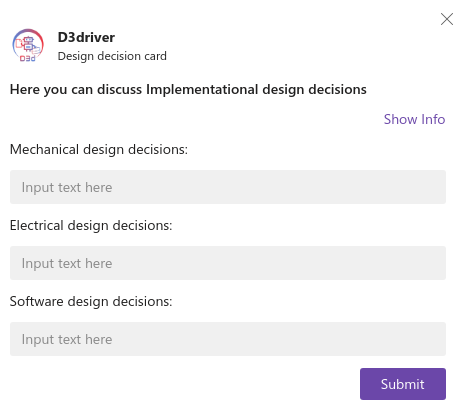
\includegraphics[width=0.7\linewidth]{figures/decisiontemplate-implementation}
\caption{Example adaptive card of Implementation phase}
\label{fig:decisiontemplate-implementation}
\end{figure}

In addition to the above design techniques, the bot is designed to use as less commands as possible to overcome the disadvantages of continuous command usage(like pointed out during the research of existing bots). The evaluation of the existing bots has also shown that in the existing designs, the users are expected to type a long and a complicated command that is a combination of many ASCII characters or the users need to make more that 2 mouse clicks to start the prioritized discussions. D3driver is designed to make the routine more effortless and thus with the help of Microsoft's \textit{Messaging Extensions}\footnote{https://docs.microsoft.com/en-us/microsoftteams/platform/messaging-extensions/what-are-messaging-extensions}, the bot adds a static button adjacent to the other default buttons beneath the standard formatting text-box. The D3driver can even be pinned to always stay visible and is just one mouse click away to start the prioritized discussions. An adaptive card will pop up as shown in the \ref{fig:decisiontemplate-implementation} upon clicking the D3driver messaging extension and further there are dedicated text-boxes to discuss prioritized messages(design decisions) whereas the other conversations that has no priority happen normally using the standard text-box offered by MS Teams. After submitting a decision to the group, all of them are stored in the database for later extraction. The D3driver tab will have a display of all the design decisions and other details like the member who took the decision, type of decision and the date of decision. A more thorough explanation of D3driver's working will be seen in the following chapter. 



\section{High-level architecture}
The figure \ref{fig:archibotnew} represents the high-level architecture of D3driver. The components of the architecture diagram are as follows:


\begin{itemize}
\item \textbf{Users} --- They symbolize the group members of a collaboration tool. The users converse with the other group members via the collaboration tool. They are the end users of D3driver. 

\item\textbf{ Collaboration tool} --- Microsoft Teams is picked as the collaboration tool for this implementation. This tool helps users to communicate with each other by means of allowing them to form teams and channels. This tool also has a rich set of conversational, productive bots that aid the users in their routine activities. This tool serves as a medium for sending and receiving messages to and from the users. Note: MS teams will come into picture once again after the bot has been hosted by Microsoft Azure. Teams is responsible for creating an important file along with logo icon-files to finally use the bot. This details of which will be discussed in the implementation chapter.

\item \textbf{Channel connector} --- A connection link between the Microsoft teams and D3driver is none other than the channel connector. To be able to deploy D3driver in the bot studio of MS teams, one must register it with Microsoft Azure bot service. Microsoft Azure has a set of approved channels. The developer must set the bot up with the appropriate channel available in Microsoft Azure. In this case, the bot should be configured with Microsoft Teams. This means the D3driver will be able to talk to users via Microsoft Teams. This connector is responsible for forwarding user’s incoming messages to the bot’s endpoint appended with the standard endpoint of MS Teams i.e. \textbf{/api/messages}. Here is an official documentation\footnote{https://docs.microsoft.com/en-us/azure/bot-service/bot-service-manage-channels?view=azure-bot-service-4.0} on how to structure bots with channels with the help of Microsoft Azure

\begin{figure}[h]
\centering
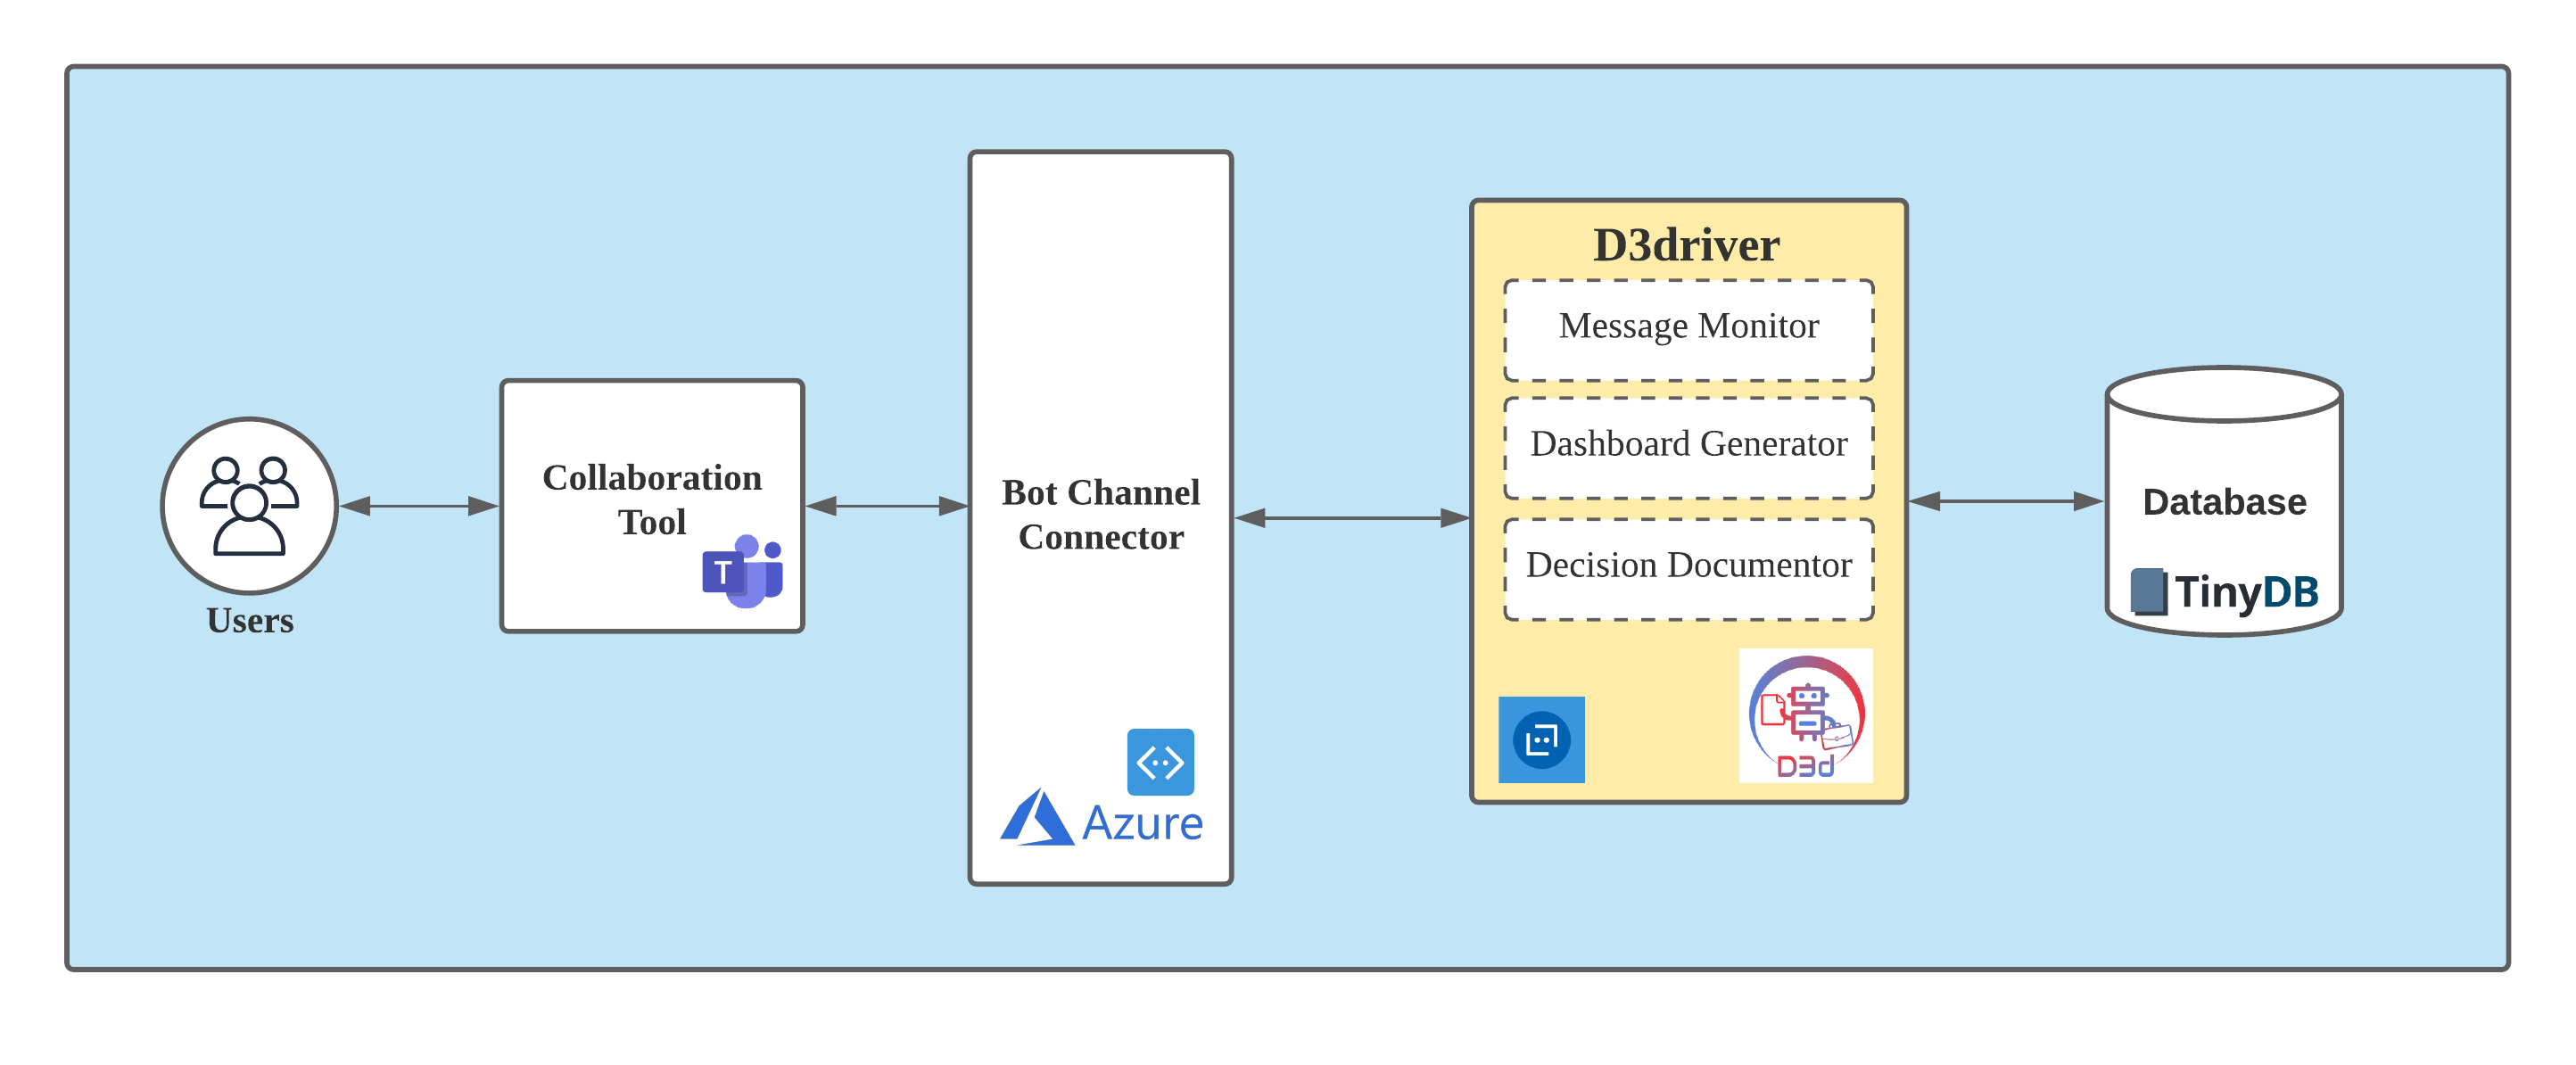
\includegraphics[width=1.1\linewidth]{figures/archibotnew}
\captionsetup{justification=centering}
\caption{ High-level bot architecture}
\label{fig:archibotnew}
\end{figure}


\item  \textbf{Bot Framework v4} --- Azure Bot Service offers a complete toolkit required to build bots, for example the popular Bot framework SDK. This framework is the core of D3driver and is the main element for developing any MS Teams bot. The framework provides many schema and this implementation will use cards schema. Card schema is the representation of interactive adaptive cards in the application-level, that can be used inside a group chat. After the bot development, the developer is required to create a new bot service by providing all the desired data. Information like name of the bot, developer location, Bot template(v4), Bot ID and password etc should all be mentioned during the registration. This will help Azure to create the bot service and deploy the bot to the cloud. After successful deployment, the developer will prepare all the necessary code files to deploy. All the files should be zipped up i.e, the python files(app.py), dependency files(requirement.txt) etc. The deployment and the channel connector configurations should make the bot available inside MS teams bot studio. Once again the official documentation for this can be seen here\footnote{https://docs.microsoft.com/en-us/azure/bot-service/abs-quickstart?view=azure-bot-service-4.0}

\item \textbf{Database} --- This is the storage component in the architecture. This serves as the persistence layer for D3driver. The incoming decisions should be stored for later retrieval and hence it would require a simple database for that purpose. TinyDB is written in python and can be easily extended to make use of custom storage. The main function of the database is to store the details like channel name, sender’s name, decision name and date etc. It can be devised to store any schema that a developer would design. After storing, it can be queried to display any data the developer wants to display on the D3driver tab.

\end{itemize}



\section{Work-flow of D3driver}

This section describes the step-by-step working of the D3driver by means of a flowchart as shown in figure \ref{fig:d3dflowchartpng}. The flowcharts depicted has 3 parts. The left hand side of the flowchart denotes the main working procedure of the D3driver using messaging extension. The central part of the flowchart depicts the process of channel initialization and the right hand side of the flowchart depicts the operations that can be performed in the D3driver tab. As soon as D3driver is installed to a channel in MS Teams, two processes will take place. 1) the D3driver's Messaging Extension will be installed and 2) D3driver's Configurable Tab will be installed. The channel initialization is done by invoking the D3driver. The bot will post a card where it asks the users to choose from one of the V-model phases. Any user selects a suitable V-model phase which is required according to their project. After selection, appropriate messages will be posted by D3driver in the group like which V-model phase has been selected and the name of the user who made this choice. 

After a V-model process is selected, the D3driver’s messaging extension(button) can be clicked to start a conversation related to design decisions. Upon clicking, an adaptive card pops up with three other input fields and their names are dependent on the V-model phase chosen for the team/project during channel initialization. The user can make use of those intended fields to discuss design decisions. After a decision is typed, the users can click on the ``submit button" within the card. Upon clicking the submit button, the typed decision is posted into the channel window. The typed decision also appears in the form of a card with name of the decision type, name of the decision maker, date of decision and the actual decision itself. This way, all design decisions are sorted from the other normal conversation material in the group chat. All these cards are saved into the D3driver's database.

The right most part of the flowchart denotes the visualization of all the saved decisions. The purpose of having a D3driver tab is to display all the decisions in one place. After the decision cards were exchanged, all the information is saved to the database and is rendered as a HTML page on the D3driver tab. The work flow of this is also simple. Any user who wants to take a look at all the decisions that has been discussed can click on the designated D3driver tab of a channel(There will be separate D3driver tabs for different channels and will contain the information that is regarded to the respective channel only). In the tab, a dashboard can be viewed with the type of channel initialization, decision type, date, decision maker etc. A search box functionality is designed to filter the desired decision card. A sort button functionality is designed to sort the decisions according to the date. A button that allows the users to download a copy of all the information present in the tab is designed. Finally, a button to view the metadata of that channel's decision cards is designed.

\begin{figure}
\centering
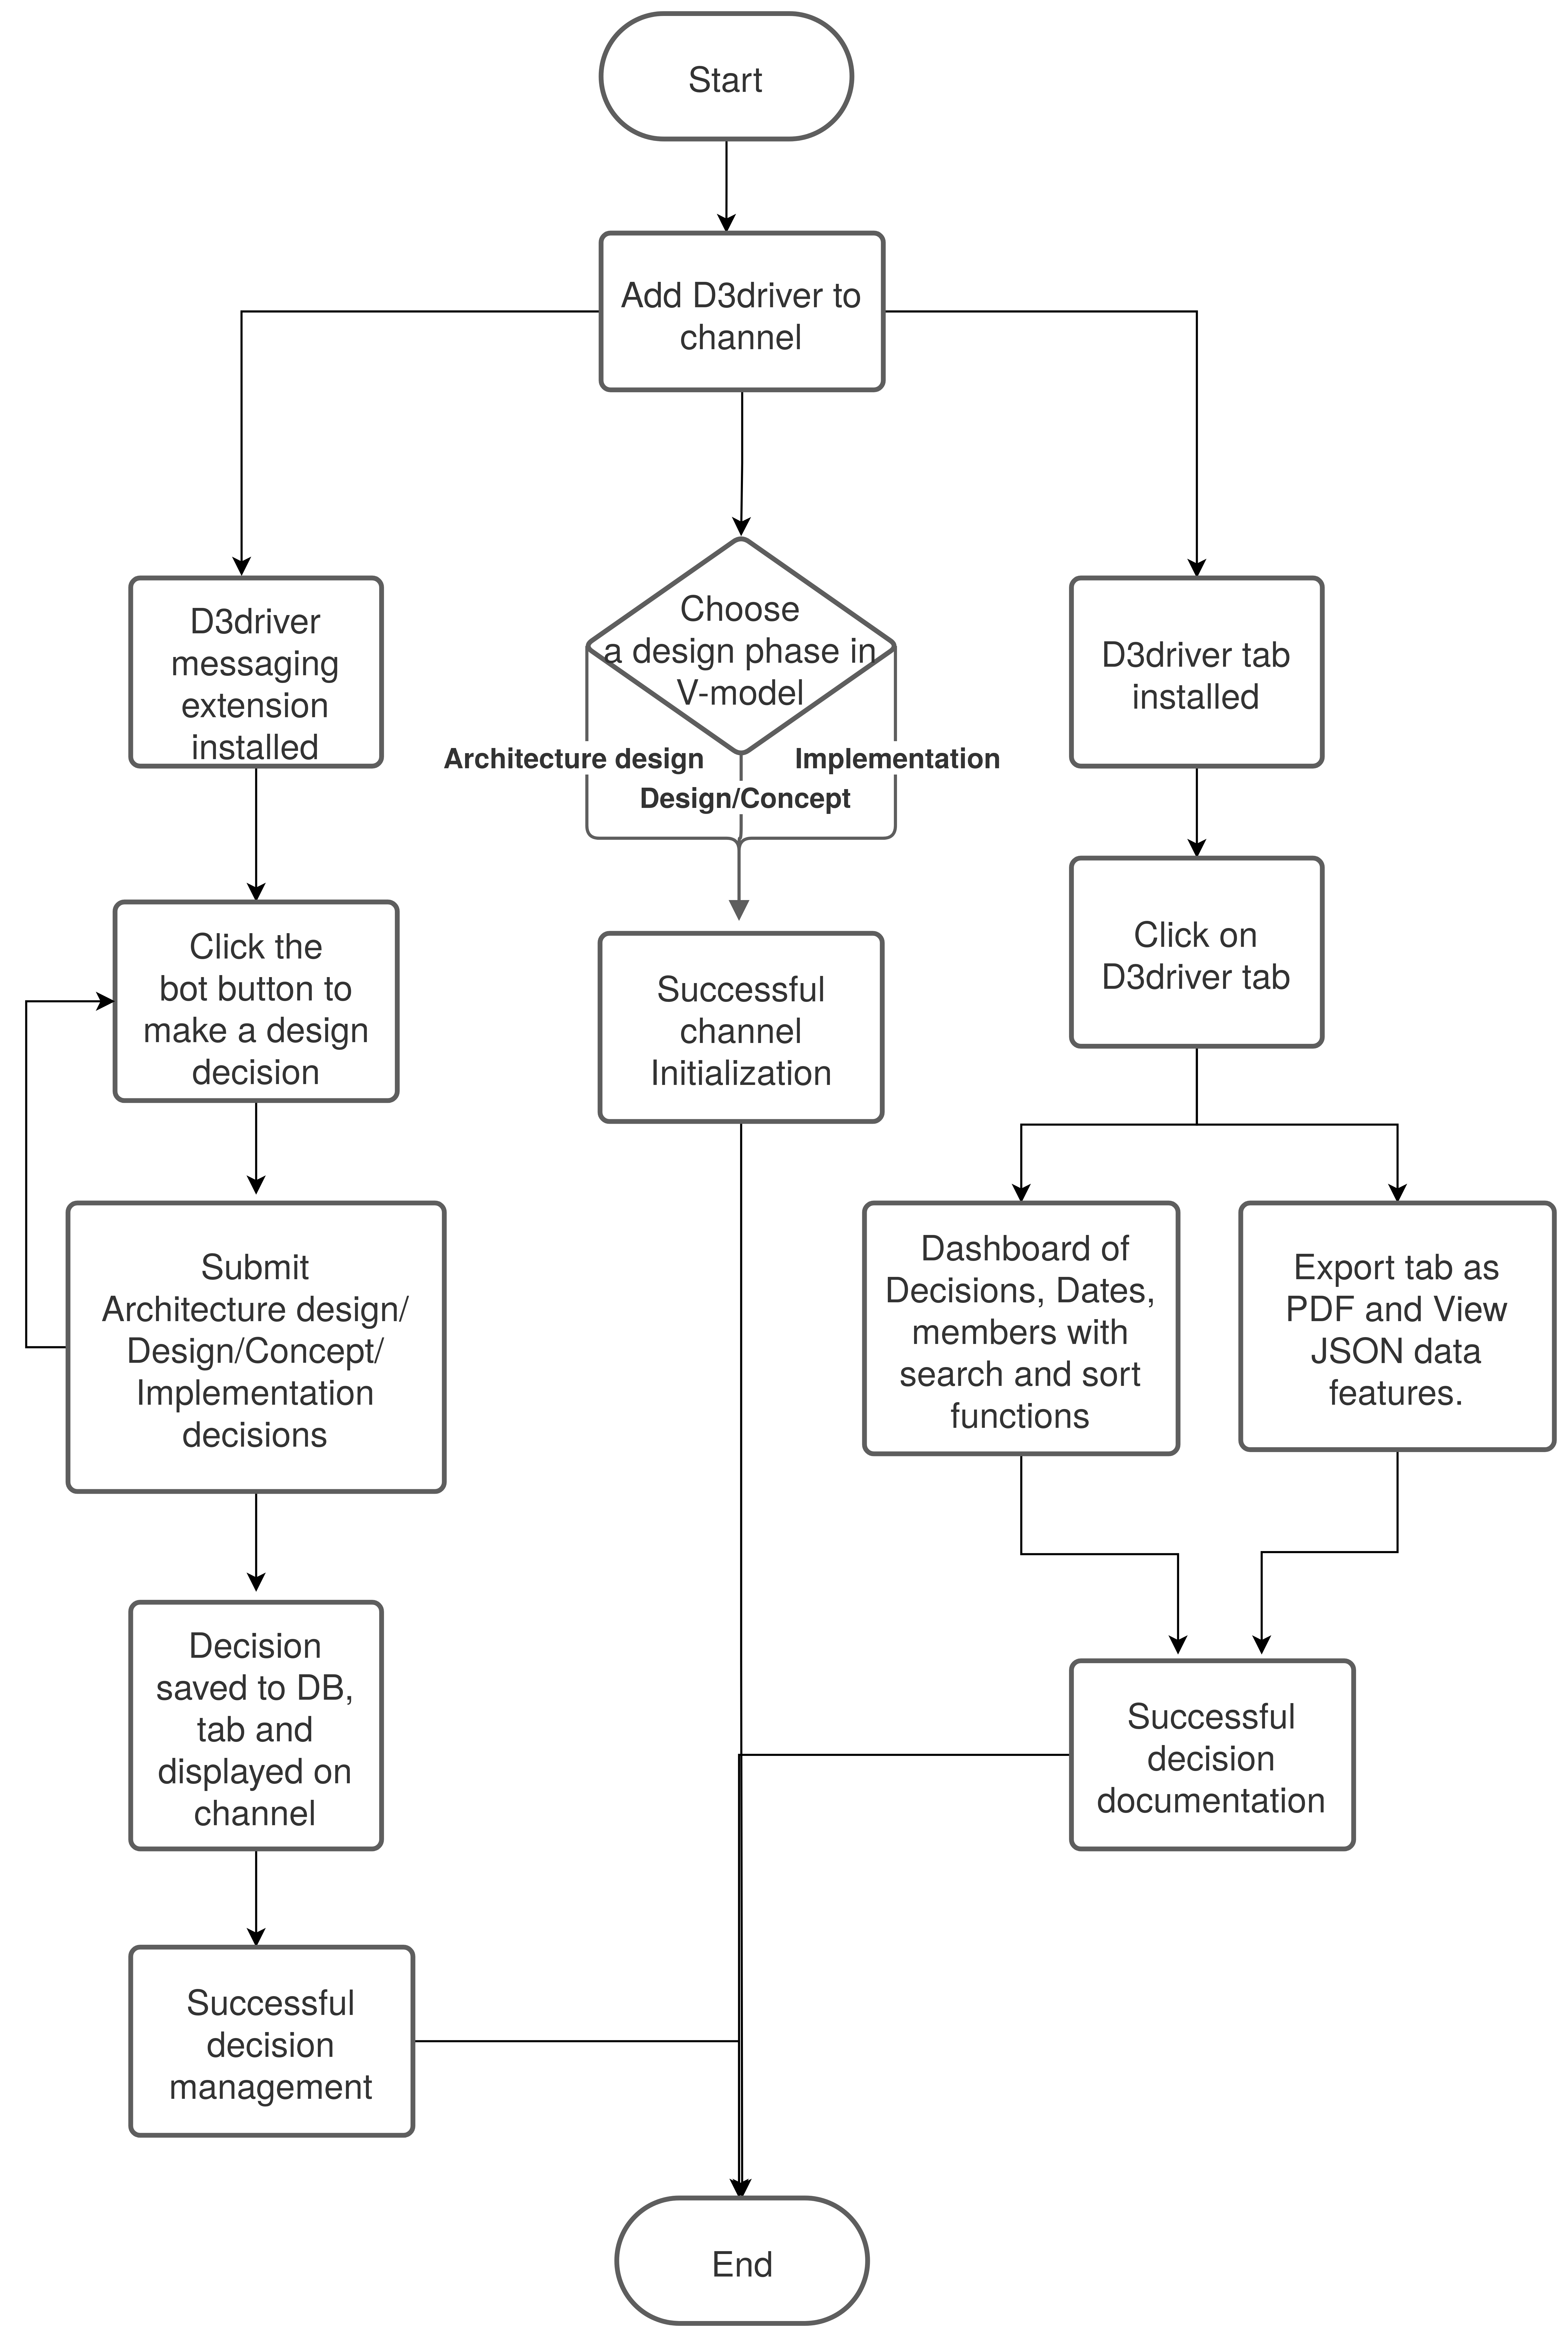
\includegraphics[width=1\linewidth]{figures/d3dflowchartpng}
\caption{Workflow of D3driver}
\label{fig:d3dflowchartpng}
\end{figure}


\section{Technologies and Applications}

The choice of technologies and applications that will be used for the implementation are listed in this section:

\begin{itemize}
\item  Microsoft Teams --- The D3driver app package is designed and developed in such a way that it can be integrated to any collaboration tool but this thesis implementation focuses on hosting the bot in Microsoft teams hence this app is the obvious choice.

\item  Microsoft Azure --- This cloud service seems to be the best to work with Microsoft teams and also the platform ensures a great collection of bot framework features. The open-source bot framework SDK v4 is an ideal development toolkit for this implementation.

\item ngrok\footnote{https://ngrok.com/docs} --- is a tunneling tool that helps users to expose their local-host server to the internet. This is a free software that can be downloaded on the system. ngrok uses either the default HTTP port or an explicit port number can be mentioned such that ngrok exposes that local port.

\item Python SDK version 3.7\footnote{https://www.python.org/} --- One of the popular programming languages that makes use of an interpreter making it an interpreted, high-level language. This is used as the main developing language for D3driver because it has simpler syntax, easy usage, can be executed faster and works well for prototyping software.

\item TinyDB\footnote{https://tinydb.readthedocs.io/en/latest/} --- As discussed in the architecture plan, this database will be used as decision database for D3driver. The design of the database is that it will have two tables to store channel related information and decision related information.

\item  HTML\footnote{https://www.w3.org/TR/html52/} \& JavaScript\footnote{https://devdocs.io/javascript/} --- D3driver tab uses these two technologies to render the card summary and other details. HTML to display the card information and JavaScript to make the page interactive.

\item  Visual studio code\footnote{https://code.visualstudio.com/} --- This is the best code editor created by Microsoft. Excellent features for code debugging, code review integrated with version control system(github). The biggest advantage is the availability of "Microsoft UI toolkit" extension with visual studio code specially used for bot development and management. It has some internal configurations with Azure that is done automatically for users and makes the process easier and faster.
\end{itemize}


This design is supposed to be the solution to poor or no documentation in a multi-disciplinary team. The design of D3driver aims at motivating team members to distinguish the most important design decisions from the typical conversations that they would have among their team. Designed in the best possible way to balance the simplicity, usability and functionality of the bot. The design also exhibits flexibility to choose the type of V-model process standard that the team wants to document. The design in ease of using the card with just one click is also the highlight and finally a dedicated tab to persist all the decisions together shows that the design is meant to decrease any effort of going through
the long threads of decisions in a channel.
















\chapter{Implementation details}
\label{chap: id}

This Chapter speaks about the implementation specifics of D3driver. This proof of concept demonstrates the possibility of execution of the solution idea that has been proposed in this thesis. 

\section{Overview of D3driver}
D3driver is a productivity bot that is uploaded as a custom app in Microsoft Teams tool. It is aimed at providing a feasible solution to teams that involve multiple domains while designing a product. It aids documenting design related decisions during a conversation between members from different domains. The team members discuss questions, answers, ideas, concepts, solutions, alternatives and decisions in their group chats. Since, decisions play a crucial role in product development, D3driver's features aid team members to track specifically design decisions document all the design decisions for later data retrieval. 

The installation guidelines of D3driver is first explained. Later, the usage is also briefly re-explained to get more familiar with the bot. Finally, each the development of each feature/functionality is explained along with their code snippets for better and clear understanding of the implementation of D3driver. The source code for this implementation is based on the boilerplate code available from the official Microsoft's online guide called Bot builder samples\footnote{https://github.com/microsoft/BotBuilder-Samples}

\section{D3driver Installation} 
The app package after uploading in MS Teams, D3driver's scope is within channels. The option `Add to team' can be selected to install the bot in the required channel. Once the D3driver is installed in a channel it sets up a messaging extension under the conversation area and a D3driver tab in the tab section as shown in the Figure \ref{fig:meandtabformarking}. 

\begin{figure}
\centering
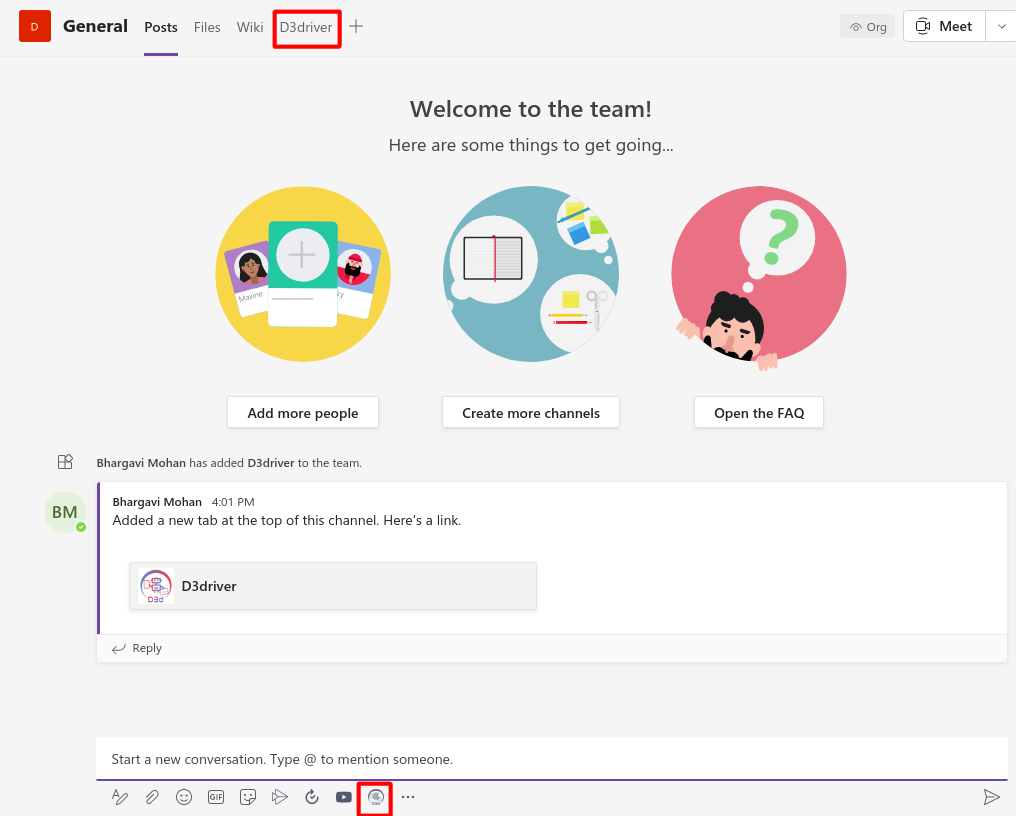
\includegraphics[width=0.8\linewidth]{figures/meandtabformarking}
\caption{Message extension icon and D3driver tab}
\captionsetup{justification=centering}
\label{fig:meandtabformarking}
\end{figure}

\subsection{Usage}
\begin{itemize}
\item Firstly, a channel should be initialized. This means a team should first select one of the three phases in V-model for accessing design decision cards. The three phases will have 3 different decision cards hence a decision card in a channel depends upon the type of initialization. The command to initialize the channel is made available in the command list. The user has to invoke the bot by typing '@D3driver' in the compose message area and the list of commands will appear. The command \texttt{init} is used to initialize the channel 

\item Once the \texttt{init} command is used to invoke the bot, D3driver replies to the channel with an initial card. A user is required to select the appropriate design phase suitable to a particular channel. 

\item Depending on the choice, the decision cards can be accessed either by invoking the bot followed by the command --- \texttt{Create card} or by hitting the messaging extension. The easiest and fastest way is to just hit the messaging extension. 

\item The different decision cards for architectural phase, design/conceptual phase and implementation phase are shown in Figures \ref{fig:fdd}, \ref{fig:dce} and \ref{fig:sw} respectively.

\item When users decide to decommission a channel, another command in the list \texttt{del} is available. By doing so, all the decisions discussed will be erased from the database. The users can choose to save the data to their local system before using \texttt{del} command by using the button "Export as PDF". It enables the members to save the entire D3driver tab as a PDF file. The filename will be in $<$channel name$>$\_$<$vphase name$>$ format. 

\end{itemize}

\section{D3driver and its components}
Firstly, when a user sends any message by invoking the bot, the control goes to the main python file \texttt{app.py} as shown in Listing \ref{lst:app.py}. It has a method called \texttt{messages()} that keeps snooping on any incoming messages and gives control to the object \texttt{BOT} of the class \newline
\texttt{TeamsMessagingExtensionsActionPreviewBot}.

\begin{lstlisting}[caption={app.py},label={lst:app.py},language=python]

BOT = TeamsMessagingExtensionsActionPreviewBot()
async def messages(req: Request) -> Response:
    # Main bot message handler.

    if "application/json" in req.headers["Content-Type"]:
        body = await req.json()
    else:
        return Response(status=HTTPStatus.UNSUPPORTED_MEDIA_TYPE)

    activity = Activity().deserialize(body)

    auth_header = req.headers["Authorization"] if "Authorization" in req.headers else ""

    invoke_response = await ADAPTER.process_activity(


        activity, auth_header, BOT.on_turn
    )

    if invoke_response:
        return json_response(
            data=invoke_response.body, status=invoke_response.status
        )

    return Response(status=HTTPStatus.OK)
\end{lstlisting}

This way, on any incoming message the control is transferred to the class. There are four important methods inside the class. 1) A method that takes control when the incoming message \texttt{init} 2) A method that takes control when the incoming message is \texttt{del} 3) A method that takes control when the messaging extension is invoked to access a decision card 4) A method that takes control when the submit button of the decision card is hit. This means that there is one method for each of the three commands and one method for submitting the decision card(this method is explained in the end, after decision cards are also discussed). These methods are explained in detail along with the details of the commands in the next section .
\subsection{Commands}
 There are 3 useful commands that come handy while using this bot. \texttt{init} , \texttt{del} and \texttt{Create card} are shown in Figure \ref{fig:commands}. The result of typing "@D3driver" followed by either of the commands is discussed one-by-one in sub sections \ref{init} , \ref{del}, \ref{me}.



\subsubsection{\textbf{init}}
\label{init}
When a channel needs to be initialized, the control jumps to the method  \texttt{on\_message\_activity()} of class \texttt{TeamsMessagingExtensionsActionPreviewBot}. The following code snippet in Listing \ref{lst:initmethod} explains how this request is handled. The variable \texttt{text\_command} checks if the \texttt{D3driverinitcommand} is assigned the value \texttt{init}, if all the conditions meet, then the V-model phase selection card is posted in the channel. The card offers the channel members to choose the type of initialization that is required for their channel as shown in the Figure \ref{fig:vphasecard}. 

\begin{lstlisting}[caption={init command handling},label={lst:initmethod},language=python]
elif text_command == D3driverinitcommand:
                        #vphase = 'Model-based'
                result = database.find_channel_exists(channel_id)
                if(len(result) == 0):
                    card = create_vphase_card_editor()
                    task_info = TaskModuleTaskInfo(
                    card=card, height=450, title="Design decision card", width=500
                        )
                    message = MessageFactory.attachment(card)
                    response_id = await turn_context.send_activity(message)
\end{lstlisting}


\begin{figure}[h]
\centering
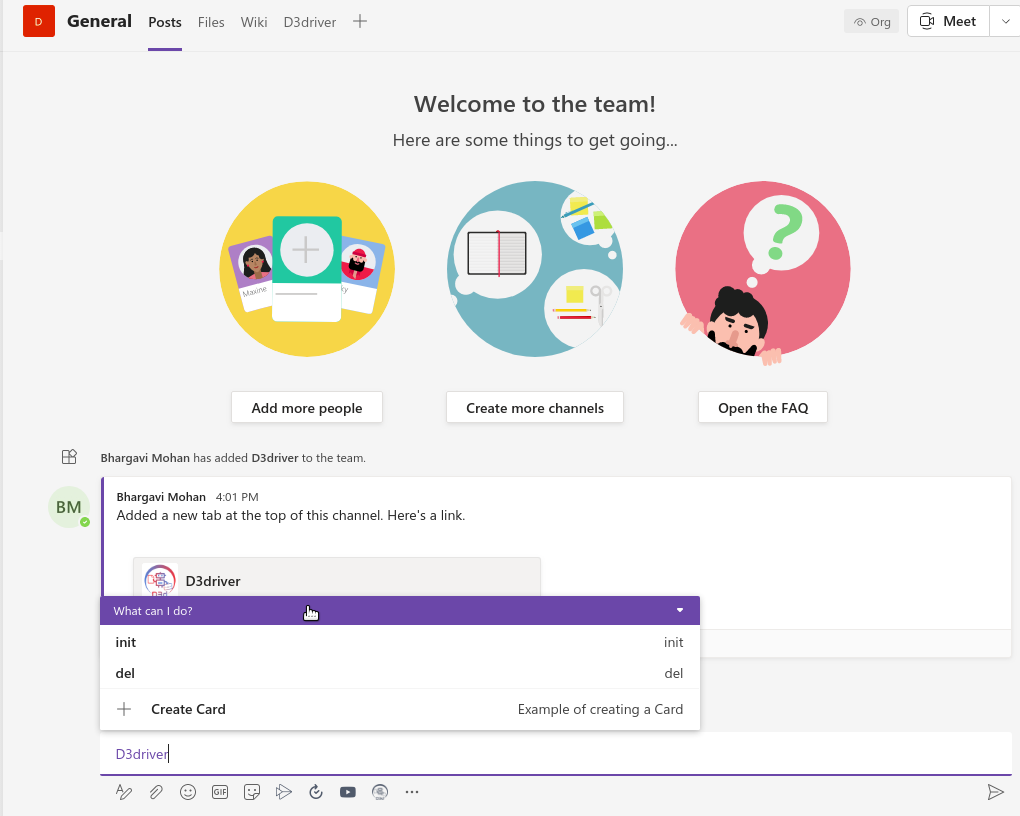
\includegraphics[width=0.7\linewidth]{figures/commands}
\captionsetup{justification=centering}
\caption{Commands}
\label{fig:commands}
\end{figure}
 
 
\begin{figure}[h]
\centering
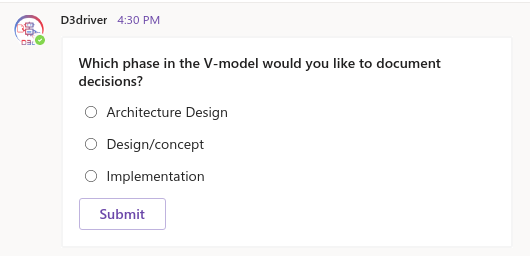
\includegraphics[width=0.7\linewidth]{figures/vphasecard}
\captionsetup{justification=centering}
\caption{V-model phase selection card}
\label{fig:vphasecard}
\end{figure} 


The Listing \ref{lst:vphasecard} shows how the V-model phase card is created. It defined the \texttt{action} section and indicates that an action has to be taken when the choices are submitted. The \texttt{body} section defined some of the text formatting definitions and the \texttt{choices} that lists the available choices that are part the card. 

\begin{lstlisting}[caption={V-model phase card},label={lst:vphasecard},language=python]
def create_vphase_card_editor(
    user_text: str = None,
    is_multi_select: bool = False,
    option1: str = None,
    option2: str = None,
    option3: str = None,
) -> Attachment:
    return CardFactory.adaptive_card(
        {
            "actions": [
                {
                    "data": {"submitLocation": "messagingExtensionFetchTask", "type" : "vmodelinit"},
                    "title": "Submit",
                    "type": "Action.Submit",
                }
            ],

                "body": [
                    {
                    "text": "Which phase in the V-model would you like to document decisions?",
                    "type": "TextBlock",
                    "weight": "bolder",
                    "wrap": True,
                },
                    {
                        "choices": [
                            {
                                "title": "Architecture Design",
                                "value": "Architecture Design"
                            },
                            {
                                "title": "Design/concept",
                                "value": "Design/concept"
                            },
                            {
                                "title": "Implementation",
                                "value": "Implementation"
                            }   
                        ],
			"id": "Choices",
                    	"isMultiSelect": is_multi_select,
                    	"style": "expanded",
                    	"type": "Input.ChoiceSet",
                    },
                ],
		        "type": "AdaptiveCard",
            	"version": "1.0",
            }
    )
\end{lstlisting}


\subsubsection{\textbf{del}}
\label{del}

This command is used in two scenarios. One is when the users decide that they no more need D3driver in their channel, it can be uninstalled by deleting the data present. An other likely scenario is when the users want to re-initialize the channel because they decide to use a different V-model phase for their project. If the team members would want to discuss a different set of design decisions, then users have to use the command \texttt{del} to reset their type of initialization. The control of the program is given to a different block in the method \texttt{on\_message\_activity()} as shown in Listing \ref{lst:delmethod}. The variable \texttt{text\_command} checks if the \texttt{D3driverdelcommand} is assigned the value \texttt{del}. If the conditions are met, then the records of this channel and decisions are all deleted from the database. A message is posted on the channel informing the successful deletion.
 
\begin{lstlisting}[caption={del command handling},label={lst:delmethod},language=python]
elif text_command == D3driverdelcommand:
                database.delete_channel(channel_id)
                database.delete_decision(channel_id)
                reply = MessageFactory.text(
                "This channel is no more initialized. All the design decsions(if discussed) has been deleted from the database. Plase click on 'Export to PDF' button in D3driver tab to save all the data to your local device. To re-initialize the channel, please enter "
                "the init command"
                )
                await turn_context.send_activity(reply)
\end{lstlisting}


\subsubsection{\textbf{Create card command / click on Messaging extension}}
\label{me}
The \texttt{Create card} command triggers the messaging extension that is configured for D3driver which means choosing the \texttt{Create card} command and clicking on the D3driver's messaging extension has the exact same effect. The control is transferred to the same method in the code and D3driver reacts to both the events in the same way. There needs to be a little background knowledge on how it is possible to incorporate messaging extension service in the D3driver.  

The Bot Framework SDK provides developers all the necessary tools, \textbf{adaptive cards}, messaging schema and communication protocols. To be able to use the SDK, a developer has to register the bot in the bot framework. The developer needs to provide some information during the registration like a name for the bot, optional endpoint etc. A Bot ID and password is generated at the end of the registration which will be required later. The bot registration of D3driver is shown in the Figure \ref{fig:botreg} and this is how the messaging extension is set up for D3driver.

\begin{figure}[h]
\centering
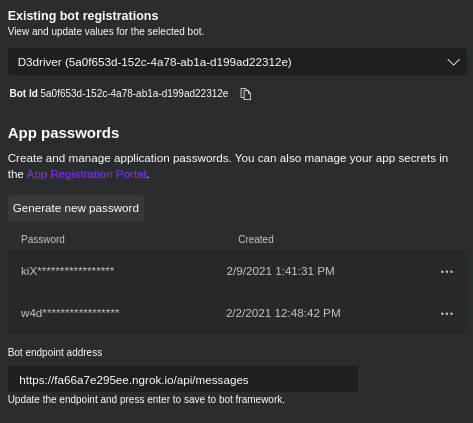
\includegraphics[width=0.8\linewidth]{figures/botreg}
\captionsetup{justification=centering}
\caption{Bot registration}
\label{fig:botreg}
\end{figure}


In general, an action based messaging extension provides the team members with a popup. This popup can either gather information from the members or display a piece of information to the members. The gathered information is then inserted into the channel. The purpose of messaging extension in D3driver is to access decision cards and gather design decisions to be documented when any user inputs the decisions in the intended text-box area. Likewise, all the members of the channel can access decision cards to exchange design decision information and this is enabled by having the messaging extension configured.  After the user hits submit button, the web service hosted by the bot framework is returned by posting the decision card to the channel. 

Observe the Listing \ref{lst:fetchtask}. The control of the program is now transferred to a different method i,e. to
\texttt{on\_teams\_messaging\_extension\_fetch\_task()}. This method examines which type of initialization a particular channel has and sends appropriate cards accordingly. The variable \texttt{result} is checked if it holds the value ``Architecture
Design" or ``Design/Concept" or ``Implementation" and three different cards namely ``create\_ad\_adaptive\_card\_editor()" or ``create\_dc\_adaptive\_card\_editor()" or ``create\_imp\_adaptive\_card\_editor()" are posted to the channel depending on the value of \texttt{result}. The method also performs certain database operations to check if the channel is already initialized, if yes, relevant message is posted on the channel else requested card will be rendered. 

\begin{lstlisting}[caption={messaging\_extension\_action\_preview\_bot.py},label={lst:fetchtask},language=python]
 async def on_teams_messaging_extension_fetch_task(
        self, turn_context: TurnContext, action: MessagingExtensionAction
    ) -> MessagingExtensionActionResponse:
        if turn_context.activity.conversation.conversation_type != 'personal':
            channel_id = turn_context.activity.channel_data['channel']['id']
            conversation_id = turn_context.activity.conversation.id #to distinguish 'Generals' of different teams
            channel_name = turn_context.activity.conversation.name
            if channel_name is None:
                channel_name = 'General'
            result = database.find_channel_exists(channel_id)
            if(len(result) == 1):
                if(result[0]["channel"]["vphase"] == 'Architecture Design'):
                    card = create_ad_adaptive_card_editor()
                    task_info = TaskModuleTaskInfo(
                        card=card, height=450, title="Design decision card", width=500
                    )
                    continue_response = TaskModuleContinueResponse(value=task_info)
                    return MessagingExtensionActionResponse(task=continue_response)
                elif(result[0]["channel"]["vphase"] == 'Design/concept'):
                    card = create_dc_adaptive_card_editor()
                    task_info = TaskModuleTaskInfo(
                        card=card, height=450, title="Design decision card", width=500
                    )
                    continue_response = TaskModuleContinueResponse(value=task_info)
                    return MessagingExtensionActionResponse(task=continue_response)
                elif(result[0]["channel"]["vphase"] == 'Implementation'):
                    card = create_imp_adaptive_card_editor()
                    task_info = TaskModuleTaskInfo(
                        card=card, height=450, title="Design decision card", width=500
                    )
                    continue_response = TaskModuleContinueResponse(value=task_info)
                    return MessagingExtensionActionResponse(task=continue_response)
            else: 
                reply = MessageFactory.text(
                "Hi there! Please initialize your channel before accessing the cards by using the init command." 
                )
                await turn_context.send_activity(reply)
        else:
            reply = MessageFactory.text(
            "***D3driver*** is pleased to help you with decision cards in your required channels. Please access the bot using the default commands in any channel. ***Happy Documenting!***"
            )
            await turn_context.send_activity(reply)
\end{lstlisting}

Some of the important inbuilt classes and their object instances of the Bot framework SDK that is operating in Listing \ref{lst:fetchtask} is explained in the following sub sections for deeper understanding.
\raggedbottom
\paragraph{Turncontext}
By passing the class \texttt{TurnContext} as argument in the function calls as shown in \ref{lst:fetchtask}, it means new instance of the TurnContext class can be created. An object of the class \texttt{TurnContext} is imported from the package \texttt{botbuilder-core} in the bot framework. This object is helpful to get the specific context during the bot's turn for processing inputs or triggering events. The context enables the developers to access all the necessary metadata and values to handle activities that are upcoming. Furthermore, another class \texttt{BotAdapter} handles the context object creation and other internal operations like authentication, sending and receiving activities from Bot service. The \texttt{TurnContext} has a couple of constructors and various properties and methods to perform specific actions.

\paragraph{MessagingExtensionAction}
This class specifies the action brought by the messaging extension. It extends a class \texttt{TaskModulerequest}. This class calls upon the request payload. \newline \texttt{MessagingExtensionAction} offers various parameters to access the user input data, user context, command ID, command context, message payload etc. It also has properties to get or set bot activity preview, get or set the ID of the command assigned by bot and gets or set message content sent as part of the command request etc. 
			
\paragraph{MessagingExtensionActionResponse}
This class returns a response to the messaging extension action. As seen in Listing \ref{lst:fetchtask} the class accepts a parameter \texttt{task} that returns the JSON for the Adaptive card to be rendered in the task module.

This marks the end of available commands in D3driver and how the corresponding function methods are called depending on the type of commands. Next, the three types of decision cards depending on the three types of initialization are discussed in the following section.

\subsection{Decision cards}
The decision cards in D3driver depends on the type of initialization. If the channel is initialized with ``Architectural design" then the card shown in Figure \ref{fig:ad} is popped up when \texttt{Create card} command is used or when messaging extension is clicked.

\begin{figure}[h]
\centering
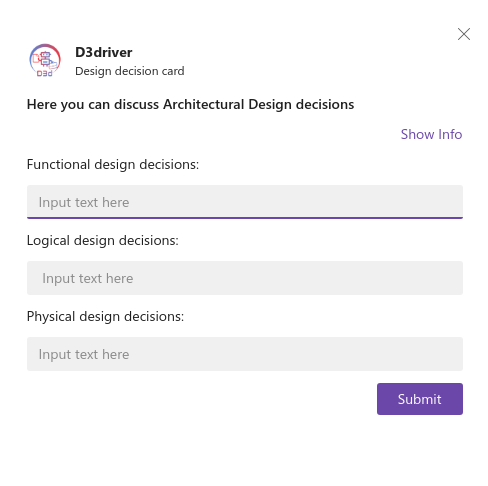
\includegraphics[width=0.6\linewidth]{figures/ad}
\captionsetup{justification=centering}
\caption{Architectural design decision card}
\label{fig:ad}
\end{figure}

The method \texttt{create\_ad\_adaptive\_card\_editor} seen in Listing \ref{lst:adcard} is called when \texttt{Create card} command is used or when messaging extension is clicked. It returns an attachment i.e. the adaptive card of type architectural design. The attachment will contain the card with a suitable `contentType'. A TypeError is caused if the card arguments are not python dicts. The adaptive cards are written in JSON format as seen in Listings \ref{lst:adcard}, \ref{lst:dccard} and \ref{lst:impcard}. The JSON has different parameters such as the field \texttt{actions} to define what has to be done when the submit button is clicked, the field \texttt{body} that defines the heading of the card, content of the sub headings and text-box areas and alignement, the field \texttt{Container} in the body indicates the meaning of each type of decision. The \texttt{Container} element introduces a toggle button called ``Show info" and ``Hide info" in UI of the decision card as seen in Figure \ref{fig:ad}. The values of the fields deliver the styling and other formatting features to appear in the adaptive cards to make them look elegant and flawless.


\begin{lstlisting}[caption={Architectural design card},label={lst:adcard},language=python]
def create_ad_adaptive_card_editor(
    user_text1: str = None,
    user_text2: str = None,
    user_text3: str = None,
) -> Attachment:
    return CardFactory.adaptive_card(
        {
            "actions": [
                {
                    "data": {"submitLocation": "messagingExtensionFetchTask"},
                    "title": "Submit",
                    "type": "Action.Submit",
                }
            ],
            "body": [
                {
                    "text": "Here you can discuss Architectural Design decisions",
                    "type": "TextBlock",
                    "weight": "bolder",
                },
                {
            "type": "ColumnSet",
            "columns": [
                {
                    "type": "Column",
                    "selectAction": {
                        "type": "Action.ToggleVisibility",
                        "targetElements": [
                            "cardContent4",
                            "showInfo",
                            "hideInfo"
                        ]
                    },
                    "verticalContentAlignment": "Center",
                    "items": [
                        {
                            "type": "TextBlock",
                            "id": "showInfo",
                            "horizontalAlignment": "Right",
                            "color": "Accent",
                            "text": "Show Info",
                            "wrap": True
                        },
                        {
                            "type": "TextBlock",
                            "id": "hideInfo",
                            "horizontalAlignment": "Right",
                            "color": "Accent",
                            "text": "Hide Info",
                            "wrap": True,
                            "isVisible": False
                        }
                    ],
                    "width": 1
                }
            ]
        },
        {
            "type": "Container",
            "id": "cardContent4",
            "isVisible": False,
            "items": [
                {
                    "type": "Container",
                    "items": [
                        {
                            "type": "TextBlock",
                            "text": "* ***Functional design decisions:*** Decisions related to functions describe functionality of the system under consideration independant of the solution.",
                            "isSubtle": True,
                            "wrap": True
                        },
                        {
                            "type": "TextBlock",
                            "text": "* ***Logical design decisions:*** Decisions related to logical architecture describes a possible implementation of the functions with defined solution principles.",
                            "isSubtle": True,
                            "wrap": True
                        },
                        {
                            "type": "TextBlock",
                            "text": "* ***Physical design decisions:*** Decisions related to the physical element describes the actual implementation, e.g. technical elements with part numbers, concrete source code, etc.",
                            "isSubtle": True,
                            "wrap": True
                        }
                    ]
                }
            ]
        },
                {"type": "TextBlock", "text": "Functional design decisions:"},
                {
                    "id": "Question1",
                    "placeholder": "Input text here",
                    "type": "Input.Text",
                    "value": user_text1,
                    "isRequired": True,
                    "errorMessage": "Any one feild is required"
                },
                
                {"type": "TextBlock", "text": "Logical design decisions:"},
                {
                    "id": "Question2",
                    "placeholder": " Input text here",
                    "type": "Input.Text",
                    "value": user_text2,
                },
                {"type": "TextBlock", "text": "Physical design decisions:"},
                {
                    "id": "Question3",
                    "placeholder": "Input text here",
                    "type": "Input.Text",
                    "value": user_text3,
                },  
            ],
            "type": "AdaptiveCard",
            "version": "1.0",
        }
    )
\end{lstlisting}



If the channel is initialized with ``Design/concept", then the card shown in Figure \ref{fig:dc} shows up and the card is developed as shown in Listing \ref{lst:dccard}. Note the descriptions of what type of decisions can be discussed using this decision template to guide the users.



\begin{lstlisting} [caption={Design/conceptual card card},label={lst:dccard},language=python]
def create_dc_adaptive_card_editor(
    user_text1: str = None,
    user_text2: str = None,
    user_text3: str = None,
) -> Attachment:
    return CardFactory.adaptive_card(
        {
            "actions": [
                {
                    "data": {"submitLocation": "messagingExtensionFetchTask"},
                    "title": "Submit",
                    "type": "Action.Submit",
                }
            ],
            "body": [
                {
                    "text": "Here you can discuss Design/conceptual decisions",
                    "type": "TextBlock",
                    "weight": "bolder",
                },
                {
            "type": "ColumnSet",
            "columns": [
                {
                    "type": "Column",
                    "selectAction": {
                        "type": "Action.ToggleVisibility",
                        "targetElements": [
                            "cardContent4",
                            "showInfo",
                            "hideInfo"
                        ]
                    },
                    "verticalContentAlignment": "Center",
                    "items": [
                        {
                            "type": "TextBlock",
                            "id": "showInfo",
                            "horizontalAlignment": "Right",
                            "color": "Accent",
                            "text": "Show Info",
                            "wrap": True
                        },
                        {
                            "type": "TextBlock",
                            "id": "hideInfo",
                            "horizontalAlignment": "Right",
                            "color": "Accent",
                            "text": "Hide Info",
                            "wrap": True,
                            "isVisible": False
                        }
                    ],
                    "width": 1
                }
            ]
        },
        {
            "type": "Container",
            "id": "cardContent4",
            "isVisible": False,
            "items": [
                {
                    "type": "Container",
                    "items": [
                        {
                            "type": "TextBlock",
                            "text": "* ***Design definition decisions:*** Decisions related to technology management,design objectives and design definition strategy, including the need for and requirements of any enabling systems, products, or services.",
                            "isSubtle": True,
                            "wrap": True
                        },
                        {
                            "type": "TextBlock",
                            "text": "* ***Design characteristics & Enablers decisions:*** Decisions related to  design characteristics for the architectural entities that ensures that the design characteristics are feasible. Design enablers such as models (physical and analytical), design heuristics, etc. are decided.",
                            "isSubtle": True,
                            "wrap": True
                        },
                        {
                            "type": "TextBlock",
                            "text": "* ***Design Alternatives decisions:*** Decisions related to assessing options for the system element to be developed using selection criteria. The most appropriate alternatives decision is made to develop the system element.",
                            "isSubtle": True,
                            "wrap": True
                        }
                    ]
                }
            ]
        },
                {"type": "TextBlock", "text": "Design definition decisions:"},
                {
                    "id": "Question1",
                    "placeholder": "Input text here",
                    "type": "Input.Text",
                    "value": user_text1,
                },
                {"type": "TextBlock", "text": "Design characteristics & Enablers decisions:"},
                {
                    "id": "Question2",
                    "placeholder": "Input text here",
                    "type": "Input.Text",
                    "value": user_text2,
                },
                {"type": "TextBlock", "text": "Design Alternatives decisions:"},
                {
                    "id": "Question3",
                    "placeholder": "Input text here",
                    "type": "Input.Text",
                    "value": user_text3,
                },  
            ],
            "type": "AdaptiveCard",
            "version": "1.0",
        }
    )
\end{lstlisting}

\begin{figure}[h]
\centering
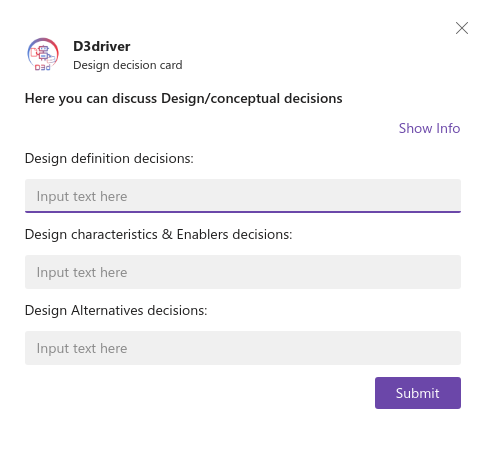
\includegraphics[width=0.7\linewidth]{figures/dc}
\captionsetup{justification=centering}
\caption{Design/concept decision card}
\label{fig:dc}
\end{figure}

If the channel is initialized with "Implementation", then the card in Figure \ref{fig:imp} appears to the users. The card is developed as shown in Listing \ref{lst:impcard}. Please observe the meanings of each decision type described to guide the users.
\begin{figure}[h]
\centering
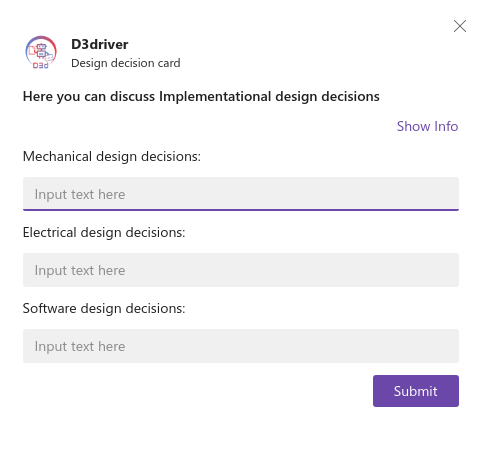
\includegraphics[width=0.6\linewidth]{figures/imp}
\captionsetup{justification=centering}
\caption{Implementation decision card}
\label{fig:imp}
\end{figure}

\begin{lstlisting} [caption={Implementation card},label={lst:impcard},language=python]
def create_imp_adaptive_card_editor(
    user_text1: str = None,
    user_text2: str = None,
    user_text3: str = None,
) -> Attachment:
    return CardFactory.adaptive_card(
        {
            "actions": [
                {
                    "data": {"submitLocation": "messagingExtensionFetchTask"},
                    "title": "Submit",
                    "type": "Action.Submit",
                }
            ],
            "body": [
                {
                    "text": "Here you can discuss Implementational design decisions",
                    "type": "TextBlock",
                    "weight": "bolder",
                },
                {
            "type": "ColumnSet",
            "columns": [
                {
                    "type": "Column",
                    "selectAction": {
                        "type": "Action.ToggleVisibility",
                        "targetElements": [
                            "cardContent4",
                            "showInfo",
                            "hideInfo"
                        ]
                    },
                    "verticalContentAlignment": "Center",
                    "items": [
                        {
                            "type": "TextBlock",
                            "id": "showInfo",
                            "horizontalAlignment": "Right",
                            "color": "Accent",
                            "text": "Show Info",
                            "wrap": True
                        },
                        {
                            "type": "TextBlock",
                            "id": "hideInfo",
                            "horizontalAlignment": "Right",
                            "color": "Accent",
                            "text": "Hide Info",
                            "wrap": True,
                            "isVisible": False
                        }
                    ],
                    "width": 1
                }
            ]
        },
        {
            "type": "Container",
            "id": "cardContent4",
            "isVisible": False,
            "items": [
                {
                    "type": "Container",
                    "items": [
                        {
                            "type": "TextBlock",
                            "text": "* ***Mechanical design decisions:*** Decisions related to mechanics like displacement, velocity, acceleration, force , torque etc.",
                            "isSubtle": True,
                            "wrap": True
                        },
                         {
                            "type": "TextBlock",
                            "text": "* ***Electrical design decisions:*** Decisions related to electronics like electric variables, voltage, current, electric field strength etc.",
                            "isSubtle": True,
                            "wrap": True
                        },
                         {
                            "type": "TextBlock",
                            "text": "* ***Software design decisions:*** Decisions related to digital information process like logical operations, algorithms, database etc.",
                            "isSubtle": True,
                            "wrap": True
                        }
                    ]
                }
            ]
        },
                {"type": "TextBlock", "text": "Mechanical design decisions:"},
                {
                    "id": "Question1",
                    "placeholder": "Input text here",
                    "type": "Input.Text",
                    "value": user_text1,
                },
                {"type": "TextBlock", "text": "Electrical design decisions:"},
                {
                    "id": "Question2",
                    "placeholder": "Input text here",
                    "type": "Input.Text",
                    "value": user_text2,
                },
                {"type": "TextBlock", "text": "Software design decisions:"},
                {
                    "id": "Question3",
                    "placeholder": "Input text here",
                    "type": "Input.Text",
                    "value": user_text3,
                },  
            ],
            "type": "AdaptiveCard",
            "version": "1.0",
        }
    )
\end{lstlisting}


This ends the discussion about the three types of cards that are made available in D3driver to discuss and document design decisions. The following sub section deals with the action taken by D3driver when the ``submit" button is clicked in each of the decision cards. The same action is taken in all three cases and is addressed as follows.

\subsubsection{\textbf{Submit button}} 
When the users insert their discussion topic in the cards and hits the submit button, the control is transferred to a method that handles this event. The four important methods of the class \texttt{TeamsMessagingExtensionsActionPreviewBot} were listed earlier. This section describes the forth method \texttt{on\_teams\_messaging\_extension\_submit\_action()} that performs two tasks. It captures the decision type, decision maker's name, date and the design decision topic and makes a database store operation to save all the information of the user that is about to submit the card. Secondly, the card is posted on the channel. The card is called ``Preview card" and this way the sender is making his decision public by clicking on submit button. The ``preview card" can be visualized in the Figures \ref{fig:fdd},\ref{fig:dce} and \ref{fig:sw}. One card from each type of initialization is depicted. The method also handles a scenario when users do not type anything and hits submit, an error message is posted. The ``preview card" is developed as shown in Listing \ref{lst:pcard}. 

\begin{lstlisting}[caption={Submit button handling},label={lst:submit},language=python]
async def on_teams_messaging_extension_submit_action(  # pylint: disable=unused-argument
        self, turn_context: TurnContext, action: MessagingExtensionAction
    ) -> MessagingExtensionActionResponse:

        channel_id = turn_context.activity.channel_data['channel']['id']
        year = str(turn_context.activity.local_timestamp.year)
        month = str(turn_context.activity.local_timestamp.month)
        day = str(turn_context.activity.local_timestamp.day)
        decisiondate = year + "-" + month + "-" + day
        channel_name = turn_context._activity.conversation.name
        if channel_name is None:
            channel_name = 'General'
        result = database.find_channel_exists(channel_id)
        if(result[0]["channel"]["vphase"] == 'Architecture Design'):
            a="Functional design decision"
            b="Logical design decision"
            c="Physical design decision"
        elif(result[0]["channel"]["vphase"] == 'Design/concept'):
            a="Design definition desisions"
            b="Design characteristics and enablers desicions"
            c="Design alterantives decisions"
        elif(result[0]["channel"]["vphase"] == 'Implementation'):
            a="Mechanical design decisions"
            b="Electrical design decisions"
            c="Software design decisions"


        user_text1 = action.data["Question1"],
        user_text2 = action.data["Question2"],
        user_text3 = action.data["Question3"],

        if(user_text1[0] == ''):
            a = ''
        if(user_text2[0] == ''):
            b = ''
        if(user_text3[0] == ''):
            c = ''
   
        memberid = turn_context._activity.from_property.name
        card = create_adaptive_card_preview(
             user_text1[0],
             user_text2[0],
             user_text3[0],
             a,
             b,
             c,
             memberid,
        )

        # db entries
        if(result[0]["channel"]["vphase"] == 'Architecture Design'):
            database.insert_decision(channel_id,channel_name,memberid,decisiondate,
            a,user_text1,b,user_text2,c,user_text3)
        elif(result[0]["channel"]["vphase"] == 'Design/concept'):
            database.insert_decision(channel_id,channel_name,memberid,decisiondate,
            a,user_text1,b,user_text2,c,user_text3)
        elif(result[0]["channel"]["vphase"] == 'Implementation'):
            database.insert_decision(channel_id,channel_name,memberid,decisiondate,
            a,user_text1,b,user_text2,c,user_text3)
        

        if (user_text1[0] or user_text2[0] or user_text3[0] != ''):
            message = MessageFactory.attachment(card)
            await turn_context.send_activity(message)
    
            return MessagingExtensionActionResponse()
        else:  
            reply = MessageFactory.text(
            "Error. No decision made"
            )
            await turn_context.send_activity(reply) 
\end{lstlisting}

\begin{figure}[h]
\centering
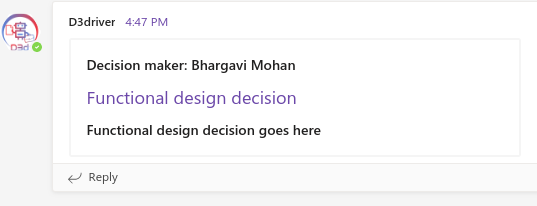
\includegraphics[width=0.7\linewidth]{figures/fdd}
\captionsetup{justification=centering}
\caption{Functional design decision posted on channel}
\label{fig:fdd}
\end{figure}

\begin{figure}[h]
\centering
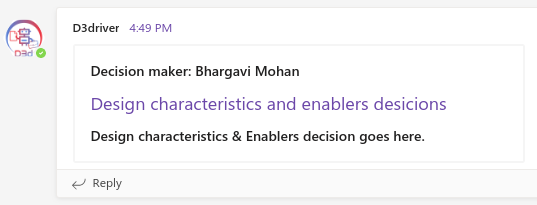
\includegraphics[width=0.7\linewidth]{figures/dce}
\captionsetup{justification=centering}
\caption{Design characteristics and enablers decision posted on channel}
\label{fig:dce}
\end{figure}

\begin{figure}[h]
\centering

\includegraphics[width=0.7\linewidth]{figures/sw}
\captionsetup{justification=centering}
\caption{Software design decision posted on channel}
\label{fig:sw}
\end{figure}





\begin{lstlisting}[caption={Preview card},label={lst:pcard},language=python]
def create_adaptive_card_preview(
    user_text1: str = None,
    user_text2: str = None,
    user_text3: str = None,
    a: str = None,
    b: str = None,
    c: str = None,
    memberid: str = None,
) -> Attachment:
    return CardFactory.adaptive_card(
        {
            "body": [
                {
                    "text": "Decision maker: {}".format(memberid),
                    "type": "TextBlock",
                    "weight": "bolder",
                },
                {
                    "text": "{}".format(a), 
                    "type": "TextBlock", 
                    "id": "Question1",
                    "color": "Accent",
                    "size": "Large"
                },
                {
                    "text": "{}".format(user_text1), 
                    "type": "TextBlock", 
                    "id": "Question1",
                    "weight": "bolder"
                },


                {
                    "text": "{}".format(b),
                    "type": "TextBlock", 
                    "id": "Question2",
                    "color": "Accent",
                    "size": "Large"
                },
                {
                    "text": "{}".format(user_text2), 
                    "type": "TextBlock", 
                    "id": "Question1",
                    "weight": "bolder"
                },
                { 
                    "text": "{}".format(c), 
                    "type": "TextBlock", 
                    "id": "Question3",
                    "color": "Accent",
                    "size": "Large"
                },
                {
                    "text": "{}".format(user_text3), 
                    "type": "TextBlock", 
                    "id": "Question1",
                    "weight": "bolder"
                },

            ],
            "type": "AdaptiveCard",
            "version": "1.0",
        }
    )
\end{lstlisting}

\section{D3driver Tab}
There are two types of tabs in Microsoft teams. 1) Static tabs and 2) Configurable tabs. Configurable tab is the focus in this thesis. It lets one to set the content of the tab dynamically each time the 
bot is added to a channel. It is nothing but a web-based HTML page generated inside a teams configurable tab. The content URL must be set properly to see a working configurable tab.(The endpoint URL can be submitted while the bot registration explained in \ref{me})

D3driver installs a configurable tab upon bot installation and the welcome page is previewed before the tab is installed as shown in Figure \ref{fig:welcomepageintab}. Once the tab is saved to a channel, all the channel specific data appears in the configured tab. The tab serves like a dashboard that displays all the design decisions discussed along with its other parameters in a team. Every channel will has its own D3driver tab and the design decisions, channel initialization type and other important information present in a tab will pertain to its respective channel. The tab will additionally have a search box, sort button and a button to export the tab as a PDF and a button to view the meta data in JSON format as shown in Figure \ref{fig:d3dtabnew}. 

\begin{figure}[h]
\centering
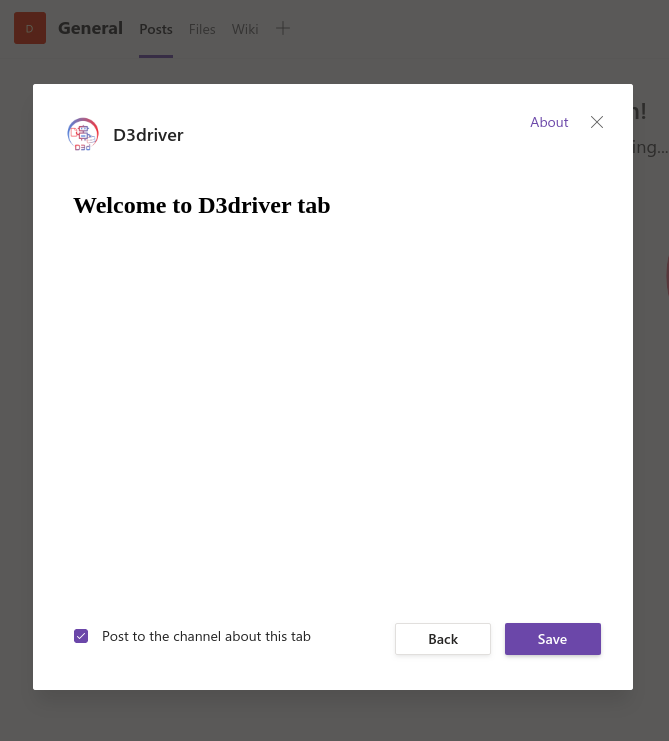
\includegraphics[width=0.6\linewidth]{figures/welcomepageintab}
\captionsetup{justification=centering}
\caption{Welcome tab}
\label{fig:welcomepageintab}
\end{figure}

\subsection{Ngrok}

The way the content is published in the tab is by using an \texttt{ngrok} tunnel. Using \texttt{ngrok}, the local endpoint is exposed to the internet hence making the HTML content available publicly. The \texttt{ngrok} providing public URL in terminal can be seen in Figure \ref{fig:ngrok}. The command to expose the local end point is right below. 

\begin{lstlisting}[language=bash]
  $ ngrok http -host-header=rewrite 3978
\end{lstlisting}

\begin{figure}[h]
\centering
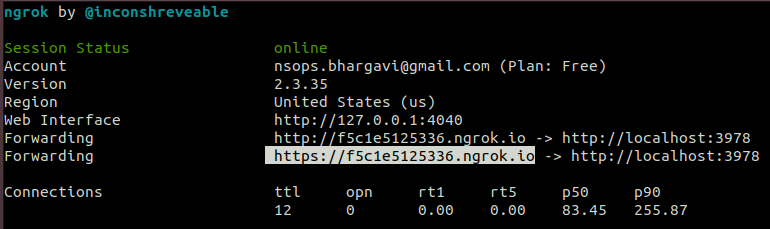
\includegraphics[width=0.7\linewidth]{figures/ngrok}
\captionsetup{justification=centering}
\caption{Ngrok endpoint}
\label{fig:ngrok}
\end{figure}


\subsection{Jinja}

Furthermore, for the purpose of templating HTML, Jinja is used. It is a web template tool for python coding. This well known template engine is responsible for populating all the mark up, source code, database records in the D3driver tab. According to the Listing \ref{lst:dash}, a page is rendered by applying \texttt{@aiohttp\_jinja2.template()} decorator to the web-handler. The method \texttt{dashboard} returns a jnja2 context. The decorator now presents the context as the web response. The python list variables \texttt{response\_obj\_tables} and \texttt{response\_obj\_decisions} capture the required data records from the database to pass it on the to the desired HTML file(dashboard.html).

\begin{figure}[h]
\centering
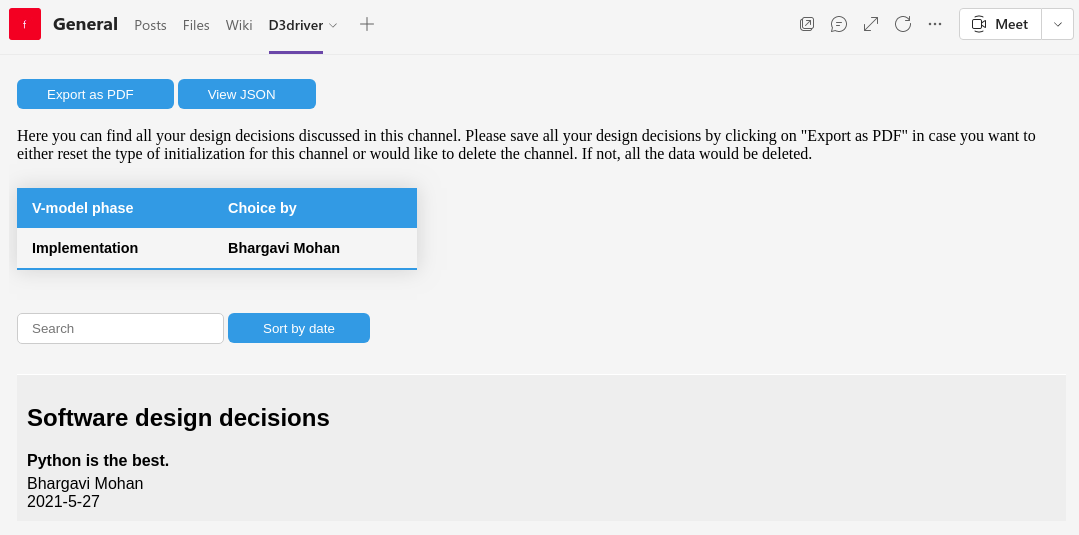
\includegraphics[width=0.9\linewidth]{figures/d3dtabnew}
\caption{D3driver tab installed in a channel}
\label{fig:d3dtabnew}
\end{figure}

\begin{lstlisting}[caption={Dashboard method},label={lst:dash},language=python]
@aiohttp_jinja2.template("dashboard.html")
async def dashboard(request):  
    try:
        param = request._rel_url.query_string
        param = param.strip('channelid=')
        response_obj_tables = database.get_channel_details(param)
        response_obj_decisions = database.get_all_decisions(param)
        ## rErroreturn a success json response with status code 200 i.e. 'OK'
        return {"decisions_list": response_obj_decisions,"tables_list":response_obj_tables}
    except Exception as e:
        ## Bad path where 
\end{lstlisting}


\subsection{AIOHTTP}

A small web server is created using \texttt{aiohttp} to support the functionality of viewing the meta data of any channel. The meta data is the raw data that is fetched from the database. The meta data is present in the JSON format. Upon click of ``View JSON" in D3driver tab, a user is redirected to their default browser to view and further work with it to edit or copy to the local system. A request handler accepts \texttt{request} as its only argument and returns the JSON data in response as shown in Listing \ref{json}.

\begin{lstlisting}[caption=View JSON button, language=python,label=json]
async def jsonreply(request): 
    try:
        param = request._rel_url.query_string
        param = param.strip('channelid=')
        response_obj_tables = database.get_channel_details(param)
        response_obj_decisions = database.get_all_decisions(param)
        return web.json_response({"decisions_list": response_obj_decisions,"tables_list":response_obj_tables})
    except Exception as e:
        return web.json_response({"error": e})
\end{lstlisting}


\subsection{JavaScript}
Two scripts have been used for the functionality of search box, sort button and export button. The library \texttt{list.js} has been used for search and date sort functions. For the export button, html2pdf javascript library has been used. A sample javascript is shown in Listing \ref{pdfjs} to observe how the PDF download script works. 

\begin{lstlisting}[language=java,caption=PDF download script,label=pdfjs]
<script>
  window.onload = function () {
    document.getElementById("download")
        .addEventListener("click", () => {
            const invoice = this.document.getElementById("invoice");
            console.log(invoice);
            console.log(window);
            var opt = {
                margin: 1,
                filename: "{{ tables_list.name | safe}}_{{ tables_list.vphase | safe}}",
                image: { type: 'jpeg', quality: 0.98 },
                html2canvas: { scale: 2 },
                jsPDF: { unit: 'in', format: 'letter', orientation: 'portrait' }
            };
            html2pdf().from(invoice).set(opt).save();
        })
}

</script>
\end{lstlisting}

\section{Database structure}
The storage for D3driver implementation is document oriented database. The data is stored as python dictionary in TinyDB. TinyDB makes use of the Python JSON module hence query to TinyDB fetches JSON data in return. TinyDB extends its support in creation of DB tables. The data modeling in tables is as same shown in Listing \ref{lst:datamodel}. Every record in the dictionary uses the name of the table as \textbf{key} and documents dictionary as \textbf{value}. Therefore, every record is stored as a \textbf{key-value} pair. The dictionary of documents contain document IDs as keys and the documents as values.

\begin{lstlisting}[caption={Data in TinyDB tables},label={lst:datamodel},language=python]
{
    'table1': {
        0: {document...},
        1: {document...},
    },
    'table2': {
        ...
    }
}...
\end{lstlisting}

For D3driver's implementation, two such tables are used. 
\begin{enumerate}
\item \textbf{\texttt{channelstable}--- } This table stores the list of all the initialized channels. It stores other important data as shown in Listing \ref{lst:Initializedchannelsanddata}. It represents one entry in the table. The \texttt{channelid} is a unique string of characters that is assigned to each channel. The \texttt{name} is the name of the channel. \texttt{vphase} is the type of initialization of that channel. \texttt{memebername} is the member who initialized the channel to \texttt{vphase} value. \texttt{date} represents the day on which the channel was initialized.
\begin{lstlisting}[caption={Initialized channels data},label={lst:Initializedchannelsanddata},language=python]
    "Initializedchannelsanddata": {
        "1": {
            "channel": {
                "channelid": "19:5642f28c1510444d9af14304ce7ce158@thread.tacv2",
                "name": "bottest",
                "vphase": "Design/concept",
                "membername": "Bhargavi Mohan",
                "date": "2021-3-10"
            }
        }
\end{lstlisting}
\item \textbf{\texttt{decisionstable}---} This table stores all the design decisions of every initialized channel. The Listing \ref{lst:des} shows a single record of this table. The \texttt{channelid} is a unique string of characters that is assigned to each channel. The \texttt{name} is the name of the channel. \texttt{membername} represents the decision maker's name. \texttt{date} represent the day on which a particular decision has been made. \texttt{decisionname\_a} , \texttt{decisionname\_b} and \texttt{decisionname\_c} corresponds the name of design decisions. This depends once again on the type of initialization of the channel. Since the channel's name is "bottest" and it's type of initialization is "\textbf{Design/concept}" - \texttt{vphase} values in Listing \ref{lst:Initializedchannelsanddata}. Hence the \texttt{decisionname\_a} , \texttt{decisionname\_b} and \texttt{decisionname\_c} would be \textbf{Design definition decisions} , \textbf{Design characteristics \& Enablers decisions} and \textbf{Design Alternatives decisions} respectively.
In the example shown in Listing \ref{lst:des}, only decision pertaining to \textbf{Design characteristics and enablers desicions} has been made, hence there is an entry against \texttt{decisionname\_b}
The records with the key names \texttt{decision\_a}, \texttt{decision\_b} and \texttt{decision\_c} will be paired with their respective values which is the actual decision topic. In the below example, \texttt{decision\_b} has some value tagged to it.

\begin{lstlisting}[caption={Design decisions table},label={lst:des},language=python]
   "Designdecisions": {
           "1": {
               "decisions": {
                   "channelid": "19:5642f28c1510444d9af14304ce7ce158@thread.tacv2",
                   "name": "bottest",
                   "membername": "Bhargavi Mohan",
                   "date": "2021-3-10",
                   "decisionname_a": "",
                   "decision_a": "",
                   "decisionname_b": "Design characteristics and enablers desicions",
                   "decision_b": "This is a place where Design characteristics and enablers desicions will be discussed",
                   "decisionname_c": "",
                   "decision_c": ""
               }
           }
\end{lstlisting}
\end{enumerate}

\section{Sequential workflow}
The sequence diagrams are a well known way of demonstrating the interactions and operations in a process. It also depicts the order of interactions or messages sent and received. 

The 3 sequence diagrams can be observed in Figure \ref{fig:initseq},  \ref{fig:create cardseq} and \ref{fig:delseq}. These basically represent the sequence of actions,reactions and exchange of messages between different functions. The figures show the sequential workflow of what happens when users invoke the bot by using the three basic commands of D3driver. The content in the rectangular boxes depicts the file names and the messages on the arrow depicts what is the action taking place. The vertical lines are called lifelines and the arrows represent asynchronous messages and replies. 



\begin{figure}[h]
\centering
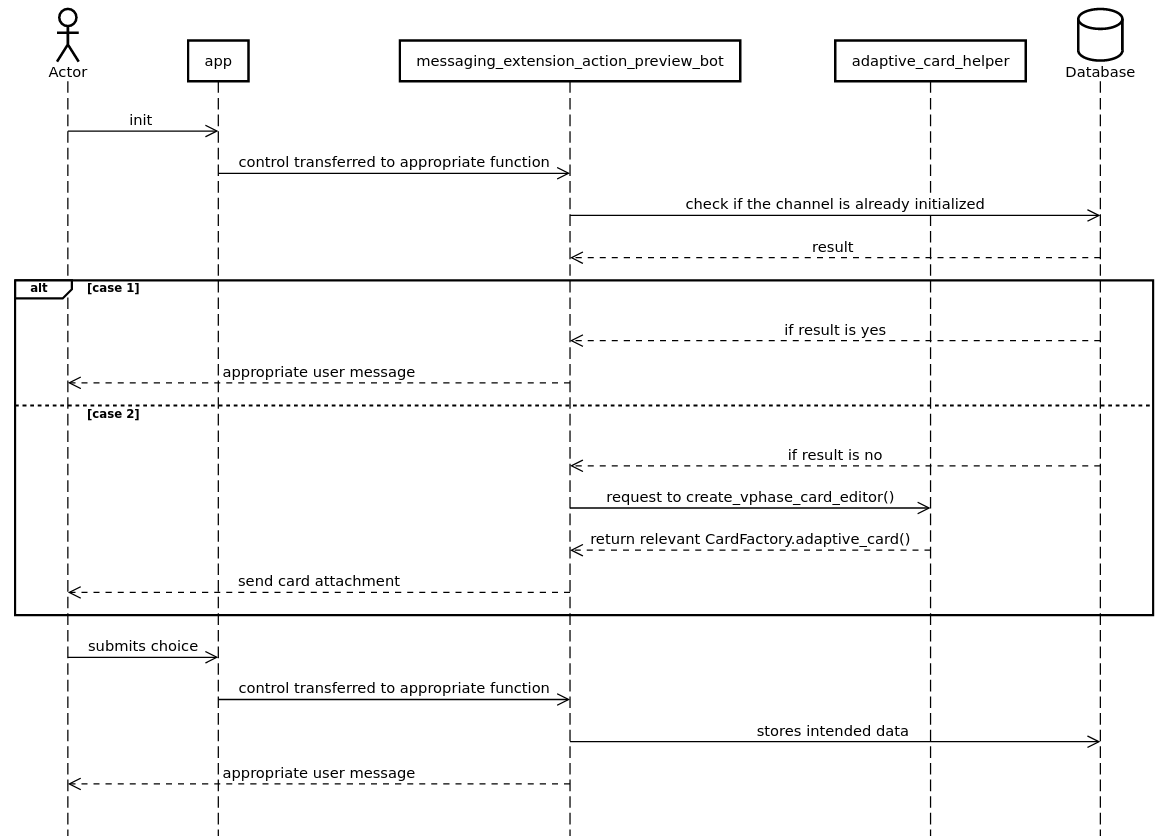
\includegraphics[width=1.1\linewidth]{figures/initseq}
\captionsetup{justification=centering}
\caption{@D3driver init}
\label{fig:initseq}
\end{figure}

In Figure \ref{fig:initseq}, the rectangular big box named ``alt" represents that there is a condition being checked. In Figure \ref{fig:create cardseq}, the big rectangular box represents that the event can happen in a loop until the user wishes to.


\begin{figure}[h]
\centering
\includegraphics[width=1.1\linewidth]{"figures/create cardseq"}
\captionsetup{justification=centering}
\caption{Create card}
\label{fig:create cardseq}
\end{figure}

\begin{figure}[h]
\centering
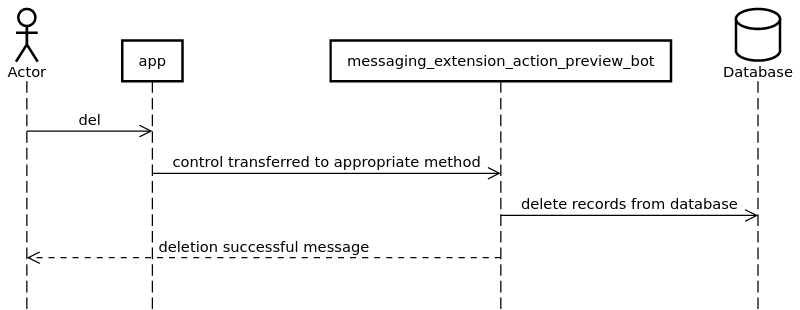
\includegraphics[width=0.9\linewidth]{figures/delseq}
\captionsetup{justification=centering}
\caption{@D3driver del}
\label{fig:delseq}
\end{figure}



\section{Manifest schema}
All the apps available in MS teams app store has to define an app manifest file. This file is a compressed file of one JSON file named as \texttt{manifest.json}, and two PNG versions of colored bot icon and an outlined bot icon of 192*192 pixels. In order to be able to upload a custom bot, the developer should prepare a zipped package of all the three. \textbf{\textit{Appstudio}}\footnote{https://microsoft.github.io/botframework-solutions/clients-and-channels/tutorials/enable-teams/4-create-app-manifest/} is already available in the MS teams app store, using which, one can easily create and edit the application manifest.

The manifest JSON file is the description of how the bot should be incorporated into Microsoft teams tool. This JSON should abide by the standard schema\footnote{https://developer.microsoft.com/en-us/json-schemas/teams/v1.8/MicrosoftTeams.schema.json} define by Microsoft. The file provides various options for attributes in its JSON body. The attributes in the JSON leads to its applicable sources such as Microsoft BOT ID, BOT password(that is generated during bot registration), a configuration URL to any static/configurable tabs. It is in this file the developer mentions if the bot should install a messaging extension , have configurable tabs , have default commands etc. There are other mandatory fields in the JSON body that should have valid values. Only when all the required fields are given the right values, the custom app(bot) can be uploaded and can be used in Microsoft teams. The app manifest of D3driver can be observed in Listing \ref{lst:manifest}. Observe the D3driver bot ID, bot full description, configuration URL that renders the D3driver tab, messaging extension configured and the scopes in which the bot is allowed to be added. 


\begin{lstlisting}[caption={Manifest file},label={lst:manifest},language=python]
{
  "$schema": "https://developer.microsoft.com/en-us/json-schemas/teams/v1.8/
  MicrosoftTeams.schema.json",
  "manifestVersion": "1.8",
  "version": "1.0",
  "id": "5a0f653d-152c-4a78-ab1a-d199ad22312e",
  "packageName": "com.microsoft.teams.samples",
  "developer": {
    "name": "UPB - Bhargavi Mohan",
    "websiteUrl": "https://dev.botframework.com",
    "privacyUrl": "https://privacy.microsoft.com",
    "termsOfUseUrl": "https://www.microsoft.com/en-us/legal/intellectualproperty/copyright/
    default.aspx"
  },
  "icons": {
    "color": "icon-color.png",
    "outline": "icon-outline.png"
  },
  "name": {
    "short": "D3driver",
    "full": "Design Decision Document driver"
  },
  "description": {
    "short": "Bot that aids documenting design decisions",
    "full": "D3driver drives the design decision documentation in the easiest way possible. This bot is exclusively designed to be used in a Mechatronics team. The design phase is an integral step in systems engineering domain. In an inter-disciplinary team, the design stage during the lifecycle of a product is extended across different phases of V-model and hence the design decisions are made throughout architectural design phase , conceptual design phase and even during the implementation phase. All these design decisions and decision makers should be distinguished from regualar or unimportant discussions that happen within a team and put together for later quick access and that is exactly what D3driver assists the users with. D3driver installs a messaging extension and a tab. The messaging extension is to access decision cards where user can choose from which phase of the V-model does the user want to document the design decisions. The tab serves like a dashboard that displays all the design decisions discusssed in a team."
  },
  "accentColor": "#FFFFFF",
  "configurableTabs": [
    {
      "configurationUrl": "https://f5c1e5125336.ngrok.io/config",
      "canUpdateConfiguration": true,
      "scopes": [
        "team"
      ],
      "context": [
        "channelTab"
      ]
    }
  ],
  "bots": [
    {
      "botId": "5a0f653d-152c-4a78-ab1a-d199ad22312e",
      "scopes": [
        "personal",
        "team"
      ],
      "commandLists": [
        {
          "scopes": [
            "team"
          ],
          "commands": [
            {
              "title": "init",
              "description": "init"
            },
            {
              "title": "del",
              "description": "del"
            }
          ]
        }
      ],
      "supportsFiles": false,
      "isNotificationOnly": false
    }
  ],
  "composeExtensions": [
    {
      "botId": "5a0f653d-152c-4a78-ab1a-d199ad22312e",
      "canUpdateConfiguration": false,
      "commands": [
        {
          "id": "createWithPreview",
          "type": "action",
          "title": "Create Card",
          "description": "Example of creating a Card",
          "initialRun": false,
          "fetchTask": true,
          "context": [
            "commandBox",
            "compose",
            "message"
          ],
          "parameters": [
            {
              "name": "param",
              "title": "param",
              "description": ""
            }
          ]
        }
      ]
    }
  ],
  "permissions": [
    "identity",
    "messageTeamMembers"
  ],
  "validDomains": [
  "7b22dd51bc42.ngrok.io",
  "*.cdnjs.cloudflare.com",
	"static2.sharepointonline.com", 
	"secure.aadcdn.microsoftonline-p.com", 
	"code.jquery.com", 
	"statics.teams.microsoft.com", 
	"*.microsoftonline.com", 
	"ajax.googleapis.com",
	"*.bing.com", 
	"*.google.com",
  	"*.statics.teams.cdn.office.net"
  ]
}
\end{lstlisting}

\section{Dockerization of D3driver}

The process of wrapping a software application along with it's dependencies inside a virtual container is the basic idea behind dockerization. The main advantage of this is that it lets the developers to build light-weight, scalable and portable software containers that makes development, testing and deployment easier. Interested readers can refer \cite{rad2017introduction} for detailed information on dockers and their advantages.

Docker image contains all the required files like dependency files, source and important libraries packed together. To build a docker image of D3driver, a \textit{Dockerfile} is created. The docker file contains the commands that will be executed when the \textit{docker-build} command is executed in the terminal as shown in Listing \ref{dbuild}.  

\begin{lstlisting}[caption={Docker build command},label={dbuild},language=bash]
docker build -f Dockerfile -t python-d3d-docker-bot .
\end{lstlisting}

The D3driver docker image creates a docker container named \textit{python-d3d-docker-bot} when the \textit{docker-run} command is executed as shown in Listing \ref{drun}. This container will have the entire D3driver application that can be run in any given environment irrespective of any operating system. Once the docker-run command is executed in the terminal, the container is started and D3driver starts running. With this, the bot can be accessed in Microsoft teams. 

\begin{lstlisting}[caption={Docker run command},label={drun},language=bash]
docker run --rm -it -p 3978:3978 -v /home/bhargavi/Documents/Masterthesis_bot2021/src/database:"/app/database" python-d3d-docker-bot
\end{lstlisting}
	
 
The implementation of D3driver is now complete. The next chapter involves the validation and verification report of the implemented software.
	

\chapter{Verification and Validation of D3driver}
\label{chap: vod}

This document details the verification and validation of D3driver. In general, verification process is done to check if all the requirements has been incorporated correctly into the product whereas validation process is to get the product tested with the stakeholder/customers to confirm that the product is according to their requirements. In this thesis, the two types of tests are done in the following way:
\begin{enumerate}
\item Verification process based on the \textit{Evaluation Criteria} that was described to screen the existing bots in section \ref{evalcrit}.
\item Validation process based on the conversation simulation between two members of the mechatronics domain. 
\end{enumerate} 

\section{Evaluation criteria - Revisited}

The Evaluation criteria that was described (based on the Requirement characteristics) in Chapter \ref{chap: eoeb} were used to check the suitability of existing bots in the context of employee motivation towards documenting design decisions. In this section, D3driver will go through the same set of criteria to get through the verification process. 

\begin{table}[h]
 \centering
\resizebox{17cm}{!}{%
\begin{tabular}{ll}
\hline
\multicolumn{1}{|c|}{\textbf{Evaluation criteria}} &  \multicolumn{1}{c|}{\textbf{D3driver}} \\ \hline
\multicolumn{1}{|l|}{Workspace - MS teams} & \multicolumn{1}{l|}{Operational in MS teams(prototype)} \\ \hline
\multicolumn{1}{|l|}{Message tagging/labeling(VDI specific)} & \multicolumn{1}{l|}{Provides decision templates in 3 important V-model design phases} \\ \hline
\multicolumn{1}{|l|}{Design decision management} & \multicolumn{1}{l|}{Clearly distinguishes normal conversations from design decisions} \\ \hline
\multicolumn{1}{|l|}{Design decision documentation} & \multicolumn{1}{l|}{Offers a separate tab to view discussed design decisions} \\ \hline
\multicolumn{1}{|l|}{Design decision Knowledge management} & \multicolumn{1}{l|}{Allows members to save a copy of the discussed decisions as PDF} \\ \hline
\multicolumn{1}{|l|}{Easy metadata retrieval} & \multicolumn{1}{l|}{ A workaround to retrieve raw data as JSON is enabled} \\ \hline
                                          
\end{tabular}
}
\captionsetup{justification=centering}
\caption{D3driver against the evaluation criteria
\label{ecr}}
\end{table}

\section{Conversation simulation using D3driver} 
The validation process was done through simulating an ``Engineering Situation" between two stakeholders using D3driver. The end goal of this exercise was to mimic the conversation as if in a product development environment. This helped in establishing helpful user stories to realize D3driver as an effective solution to the problem statement of this thesis.

The agenda of this workshop was as follows
\begin{itemize}
\item Initial setup --- A channel was created in Microsoft teams for the validation purpose. The bot D3driver was added to the channel. The supervisors(members) were also added to the channel. 
\item Stakeholder roles --- The supervisors were defined specific roles to replicate a real scenario. 
\item Design Phases --- The two members discuss some design decisions in each of the V-model phase. The stakeholder roles are re-defined in every phase.
\item Validation --- The members use all the commands and test all the features of D3driver that includes working of ``D3driver messaging extension", ``configurable D3driver tab" , ``search box", ``sort button", ``Export as PDF" button and ``View JSON" button. 
\item At the end of this workshop, the members were also given a survey of questionnaire that was based on the evaluation criteria. 
\end{itemize}

\subsection{User stories}
There are 3  V-model design phases that are taken into account by D3driver to document design decisions hence 3 scenarios are illustrated in this section. The name of the design phase and the roles defined are mentioned for each illustration. There are also member names present in the parenthesis according to their MS teams user IDs. The use case to each phase is also elaborated. To begin with, one of the members initialized the channel by invoking the bot as shown in \ref{fig:initadp}, an appropriate message sent by the bot can also be observed in the screenshot. 


\begin{figure}
\centering
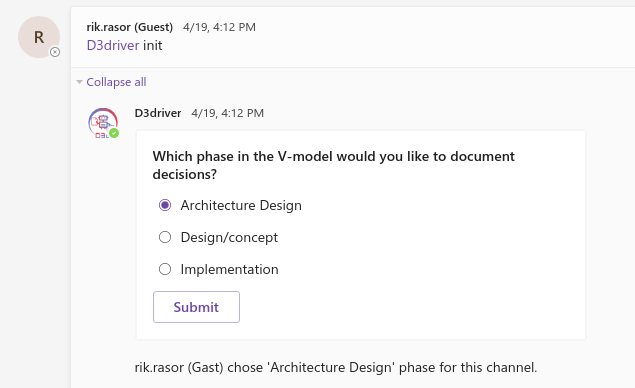
\includegraphics[width=0.7\linewidth]{figures/initadp}
\caption{Channel initialization}
\label{fig:initadp}
\end{figure}


\begin{enumerate}
\item Phase - \textbf{Architecture phase} \newline
Roles - \textbf{Product owner (st.a.pfeifer (Gast))  and Systems architect (rik.rasor (Gast))} \newline
Use case 1 - \textbf{Decision on Logical design} 

In this phase, the two members discuss in short about a logical design decision related to Voltage as shown in \ref{fig:discussionadp}. These conversations are termed as normal messages in the group chat which are of least importance. After a quick initial discussion, the team members choose to document the design decision which they think is significant. Hence, they use D3driver messaging extension to document their decision. When they submit the decision to the group chat, a decision card is posted by D3driver and is depicted in \ref{fig:lddbyd3d}.

\begin{figure}
\centering
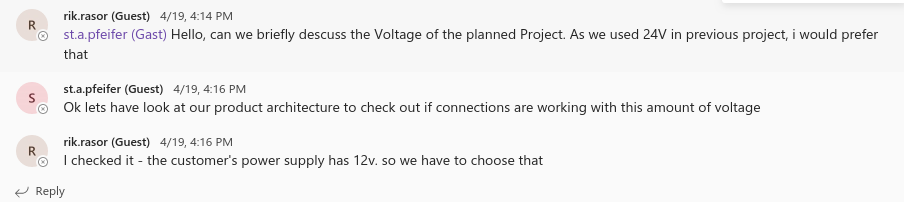
\includegraphics[width=0.8\linewidth]{figures/discussionadp}
\caption{Normal group discussions}
\label{fig:discussionadp}
\end{figure}

\begin{figure}[h]
\centering

\includegraphics[width=0.7\linewidth]{figures/lddbyd3d}
\caption{Logical design decision card}
\label{fig:lddbyd3d}
\end{figure}

\newpage

Use case 2 - \textbf{Decision on Functional design}

In the subsequent use case, the members had a brief discussion on the functionality of intended device of their planned project. One of the members inquired if the device should be connected to an app or was it sufficient to use the control on the device itself. The other member chose their preference and made a decision and documented it using D3driver as shown in \ref{fig:fddadp}


\begin{figure}[h]
\centering
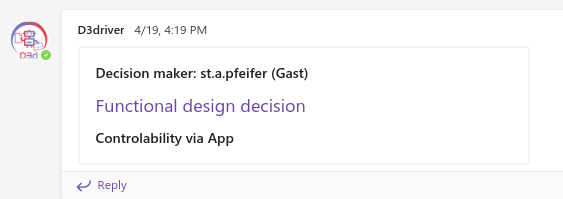
\includegraphics[width=0.8\linewidth]{figures/fddadp}
\caption{Functional design decision card}
\label{fig:fddadp}
\end{figure}

The team members wished to re-initialize the channel with a different V-model phase. Hence, they saved their previous design decisions by clicking on the ``Export as PDF" in D3driver tab as shown in \ref{fig:d3dtabadp}. The downloaded file was also viewed as shown in \ref{fig:pdffile}. They members were also able to view the metadata by clicking on ``View JSON" as shown in \ref{fig:json}. The next step was to use the delete command before re-initialization as shown in \ref{fig:delete}

\begin{figure}[h]
\centering
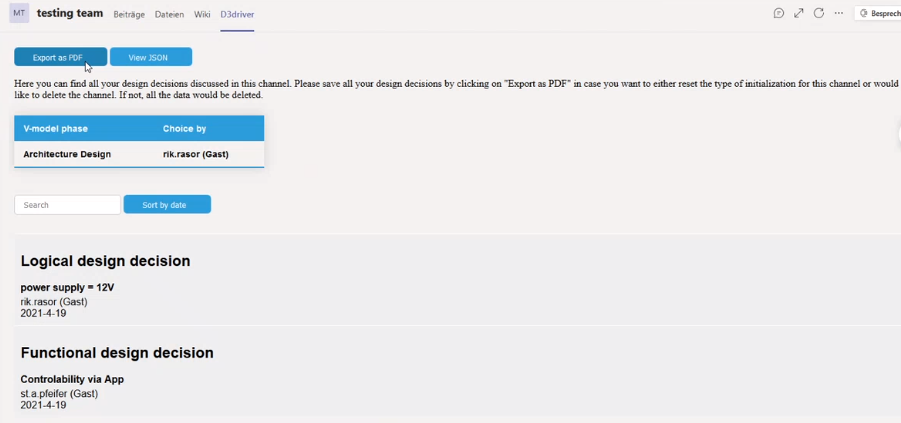
\includegraphics[width=0.8\linewidth]{figures/d3dtabadp}
\caption{D3driver tab features}
\label{fig:d3dtabadp}
\end{figure}

\begin{figure}
\centering
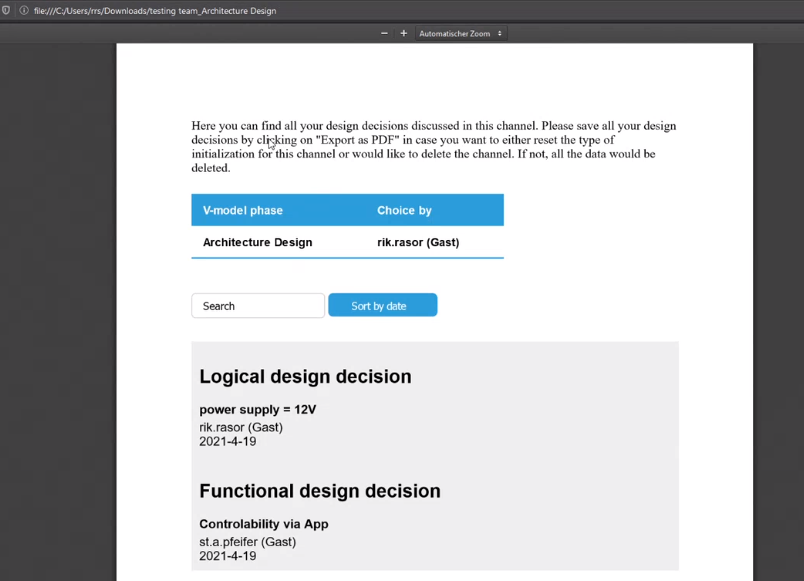
\includegraphics[width=0.7\linewidth]{figures/pdffile}
\caption{View of downloaded PDF file}
\label{fig:pdffile}
\end{figure}


\begin{figure}
\centering
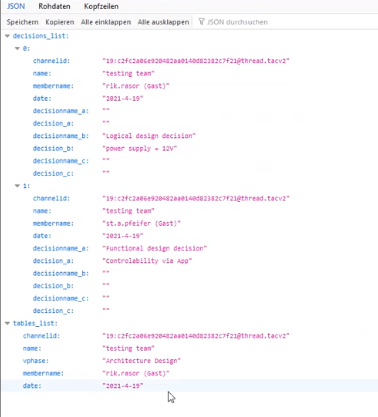
\includegraphics[width=0.7\linewidth]{figures/JSON}
\caption{JSON data view}
\label{fig:json}
\end{figure}

\begin{figure}
\centering

\includegraphics[width=0.8\linewidth]{figures/delete}
\caption{Delete command message}
\label{fig:delete}
\end{figure}



\item Phase - \textbf{Design/Concept phase} \newline
Roles - \textbf{Software Engineer (st.a.pfeifer (Gast) and Mechanical Engineer(rik.rasor(Guest))} \newline
Use case 3 - \textbf{Decision on Design alternatives}

The members once again re-initialize the channel to Design/Concept as shown in \ref{fig:initdc}. The software engineer discusses  control-ability and says that control through software is one option and a motor controller can be implemented so as to regulate the momentum and the velocity of the drives. On the other hand, a mechanical engineer mentions that the control-ability through a clutch is also a good idea. In this scenario, the team members after a discussion arrive at a design decision that they want to document. Hence, they once again use D3driver for decision documentation as shown in \ref{fig:design-alternative-decision}. 

\begin{figure}
\centering
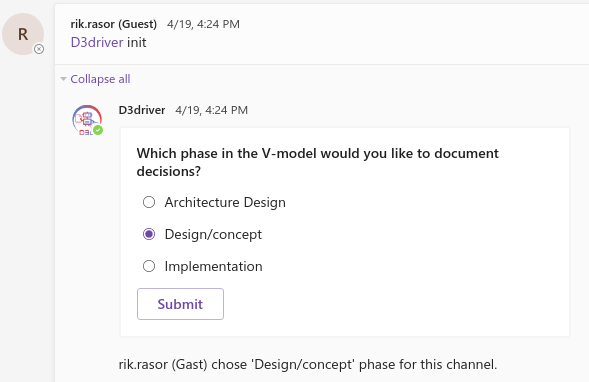
\includegraphics[width=0.7\linewidth]{figures/initDC}
\caption{Re-initialization of channel to Design/concept}
\label{fig:initdc}
\end{figure}


\begin{figure}
\centering
\includegraphics[width=0.7\linewidth]{"figures/design alternative decision"}
\caption{Design alternative decision card}
\label{fig:design-alternative-decision}
\end{figure}



\item Phase - \textbf{Implementation phase} \newline
Roles - \textbf{Two Software engineers (st.a.pfeifer (Gast) and rik.rasor (Gast))} \newline
Use case 4 -  \textbf{Decisions on software design}

At this point, the team saves the discussed decisions, deletes the current initialization and finally re-initializes for the last time as shown in \ref{fig:impleinit} to discuss implementation design decisions. The discussion during the implementation phase is related to the controller parameters. The software implementation of a Proportional–Integral–Derivative (PID) controller for the velocity control of the system was discussed. The two software engineers examine the better values to "P" and finally an experienced decision is made and the team once again uses D3driver to document the software design decision as shown in \ref{fig:software-design-decision}. As a final step, the team also utilizes the search box feature as shown in \ref{fig:search-button}. The sort button was also reviewed and the dates can be sorted in either ascending or descending order as shown in \ref{fig:sort-button}

At this stage, the validation is said to be complete. It can be implied from the user stories and screenshots of the simulation that the D3driver behaves as expected and has proved it's potential to carry out all it's tasks adequately well. The two stakeholders(supervisors) undertook a survey that sought their user experience of D3driver. The survey questionnaire was framed based on the evaluation criteria. Their responses have been recorded and can be viewed here\footnote{https://docs.google.com/forms/d/1U45XPGRnw0L9-CVKsVAX0R-FlWS4dMBfwYolZOzlVZE/viewanalytics} for reference.

\begin{figure}
\centering
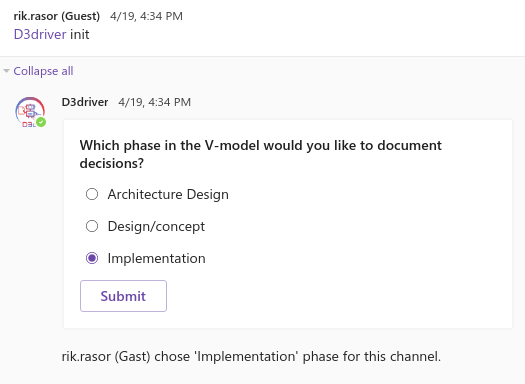
\includegraphics[width=0.7\linewidth]{figures/impleinit}
\caption{Channel initialized to Implementation}
\label{fig:impleinit}
\end{figure}


\begin{figure}
\centering
\includegraphics[width=0.7\linewidth]{"figures/software design decision"}
\caption{Software design decision card}
\label{fig:software-design-decision}
\end{figure}


\begin{figure}
\centering
\includegraphics[width=0.7\linewidth]{"figures/search button"}
\caption{Search box}
\label{fig:search-button}
\end{figure}

\begin{figure}
\centering
\includegraphics[width=0.7\linewidth]{"figures/sort button"}
\caption{Sort button}
\label{fig:sort-button}
\end{figure}

\end{enumerate}







\chapter{Conclusion and Future Enhancements}
\label{chap: cafe}

In conclusion, D3driver has been successful in reaching the goals defined for this thesis implementation. D3driver was meant to ease the design decision making process for a multi-disciplinary team like mechatronics and the bot renders all the needful functionalities to accomplish the targets. 

The thesis embarked with a notion to stress the emphasis of employee motivation especially towards documentation during a collective chat discussion in an inter-disciplinary team. Although, there were two other objectives put forward for the sake of employee motivation during the proposal phase, the scope and time limitation of the thesis had to be considered. The objective with the highest priority has been successfully implementing in the course of this thesis. The thesis in it's initial phases established the fact that collaboration is an essential component of any team especially when there are members from various domains. Teamwork, partnership and co-ordination normally happens over a collaboration tool and if that serves as an important aspect, then documenting chief facts and observations in the process is also equally important. The importance of documentation in mechatronics was discovered in parallel. At that moment, there was no system in place to handle the documentation functionality as per the need. Henceforth, it made sense to define what is lacking and what needs to be done further. This was followed by defining a problem statement. Once the problem was described, objectives and solution ideas were aligned and therefore the mission was to develop a bot preferably in MS Teams to motivate users upon documenting design decisions of mechatronics in a group chat. To this end, the background study began. The literature survey of mechatronics systems, processes, collaboration tools, decision making in mechatronics and bots in MS teams helped to channelize the research and implementation in the right direction. Thereafter, four prominent stages broke out which is as follows. 


At this point, this thesis work had the right foundation to go ahead with the first stage of evaluating existing solutions to the described problem. This phase was more of a research task to determine the pros and cons of already existing bots in a couple of known collaboration tools. This involved establishing a set of evaluation criteria based upon the requirements and objectives of this thesis work. The bots were installed and tested to see which evaluation criteria was fulfilled, followed up a summary report. This stage formed a great groundwork for further stages.  

The next two stages, design and implementation of a motivational bot represent the crux of this work. After some study on what technologies and applications would best suit the thesis specifications, the name, logo, architecture, workflow and approaches to implementation originated and the same has been explained. During the implementation stage, bot development guidance provided by official Microsoft documentation helped in prototyping D3driver and it's features. A detailed report on D3driver's installation, usage, components, intricate working has been presented. In addition, interested users can also take a look at the GitHub repository\footnote{https://github.com/bhargavimohan/Masterthesis\_bot2021} for source codes and user manual.

The final stage in this work was the verification and validation of D3driver. This stage first verifies to see if the bot meets all the required specifications and confirms that the bot can be made available to the users. D3driver was reviewed against the same set evaluation criteria that was established to review existing bots. Next, validation was done by having two members from different domains simulate engineering scenarios where design decision documentation was done with the use of D3driver. The results of this demonstration was logged and submitted in this report. With this, all the four stages of bot prototyping has been victoriously completed.

\section{Future enhancements}

Future work on D3driver can persevere in 2 different paths. One in which D3driver's current functionalities can be upgraded and another direction would be to add new innovations (other than documentation functionality) altogether. The latter has already been proposed in Chapter \ref{chap: into}. A clear conception on two more functionalities in the area of employee motivation, their problem description, objectives and solutions has also been suggested in sections \ref{pd} , \ref{obj} and \ref{si} respectively. These two were marked as secondary or optional goals in this thesis. 


For the purpose of improving the current features of D3driver, the following points can be noted.

\begin{itemize}
\item Introducing another option to the list of initialization options. Right now, there are 3 phases of V-model as initialization choices, however there could be a ``custom" choice and introducing ``custom" sub-options. With this, the users will be able to label their own decision names and will be able to document anything other than just design decisions. 

\item Designing graphs and statistics in the D3driver tab to see the total number of decisions, highest number of decisions taken by a particular member, highest number of decision types discussed and a few more useful facts and figures depending on the actual requirement in a team. 

\item The orientation of the decisions displayed in the D3driver tab can be visualized in a more refined way. There can be different layouts for each decision type with their own search and sort functionalities. This would further make the search feature optimized when there are thousands of decisions discussed. 

\item The sort functionality can also be further enhanced by introducing more sort by options like \textit{sort by members} and \textit{sort by decision type}. This would help users to generate a precise report of decision types or decision makers. For instance - \textit{sort by members} functionality would line up all the decisions taken by a particular member and when this is on display, the users can use ``Export as PDF" button to generate this report before it is refreshed.

\item At present, D3driver can be added to any channel. But this can be extended  to ``\textit{Add to meeting}" to document decisions pertaining to V-model design phases while the meeting is going on. This can help the users maintain a separate thread of design decision discussions exclusively during meetings. 

\item The database structure can be made more advanced by using a more sophisticated database other than TinyDB to handle huge records to enable scalability in production environment.

\item Finally, making D3driver a production-ready bot to deploy it in Microsoft azure is a major upgrade. This will result in an implicit performance upgrade of not having to use \textit{ngrok} technology and can avoid frequent \textit{ngrok url} update in the code. This would also make the bot be available to public for usage. 


\end{itemize}

Apart from the above ideas, there are some minor design advancements to be considered:

\begin{itemize}
\item A welcome card with greetings and detailed instructions on the available commands and their usage can be designed to be sent on bot start up without any user requiring to invoke the bot.

\item A special card asking deletion confirmation can be designed after using the \textit{``del"} command. Currently, the ``del" command would erase all the data when used without a warning.

\item The current version of adaptive cards in MS teams has a limitation on the radio button graphical appearance. It is visible only to the user making an option during channel initialization and the radio button appearance is not visible to other members who aren't making the choice (however, appropriate messages appear immediately on the choices made for users who do not make the initialization choice). Hence, when an update on the version of adaptive card is available, changes to reflect this design improvement can be considered. 
\end{itemize}







\bibliographystyle{literature/myalphadin}
\bibliography{literature/literature}

\rmfamily
%\chapter{Appendix}


\end{document}